% BEGIN ------------------   Version   ------------------- END %

\newcommand{\start}{February 11, 2013} % Definie la commande << start >>, à laquelle on a attribué une date.
\newcommand{\version}{\today} % Define la commande << version >>, à laquelle on a attribué ici la date d'aujoud'hui.
\newcommand{\final}{×} % Define la commande << final >>, à laquelle on a attribué une date.


% BEGIN ------------------   Classe du document   ------------------- END %

\documentclass[a4paper,11pt]{article} % Le format du papier, la taille de police d'écriture, le modèle du document.
% Classe existante: article, book, letter, beamer, amsart.

% BEGIN-------------------   Packages   ------------------- END %

\usepackage[french,english,german,italian]{babel} % Permet de sélectionner la langue, ici je vais avoir le choix entre le français, l'anglais, l'allemand, et l'italien. 
\usepackage[utf8]{inputenc} % Evite le problème des accents.
\usepackage{graphicx} % Permet d'incorporer des images.
\usepackage{geometry} % Permet de la flexbilité sur la géométrie.
\usepackage{amsfonts,amsmath,amsthm,amssymb,amscd,amsxtra} % Package pour les maths.
\usepackage{array} % Package pour dessiner des tableaux.
\usepackage{color} % Permet d'utiliser des couleurs personnalisées (black, white, red, green, blue, cyan, magenta).
\usepackage[hyperindex=true,colorlinks=true,linkcolor=black,urlcolor=black, citecolor= black, pagebackref=true]{hyperref} % Insere des liens (liens dans les indexs, colorie les liens, couleur des liens interne, couleur des hyperliens, couleur des citations, permet de faire figurer dans la bibliographie les pages où sont cités les article).
\usepackage{cancel} % Permet de barrer des éléments.
\usepackage{multicol} % Permet de mettre une partie de son document sur plusieurs colonnes.
\usepackage{latexsym} % Permet d'inserer d'autres symboles mathématique.
\usepackage{mathrsfs} % Permet d'utiliser \mathscr{}.
%\usepackage{footnotebackref} % Permet la création de liens interne à partir des footnote.
\usepackage{natbib} % Permet de changer la couleur des numéros dans la biblio.

% BEGIN --------------------  BACKREF  -------------------- END %

\newcommand{\mapolicebackref}[1]{\hspace*{\fill}\mbox{\textit {\small #1}}} % Définir un style pour les backrefs.
\renewcommand*{\backref}[1]{}
\renewcommand*{\backrefalt}[4]{
                               \ifcase #1 \mapolicebackref{}
                               \or \mapolicebackref{Cited page #2}
                               \else \mapolicebackref{Cited pages #2}
                               \fi
                               } % Pour gérer les backref dans la bibliographie.


% BEGIN --------------------  Commandes personnalisées  -------------------- END %

\newcommand{\bra}[1]{\langle{#1}|} % Definie le Bra.       
\newcommand{\ket}[1]{|{#1}\rangle} % Definie le Ket.
\newcommand{\abs}[1]{\left|{#1}\right|} % Define la valeur absolue.
\graphicspath{{./figures/}} % Permet d'aller chercher les figures, images, etc dans un dossier nommé figures.

% BEGIN --------------------  numberwithin  -------------------- END %

\numberwithin{equation}{section} % Permet de numéroter les equations suivant la section où elles se trouvent.
\numberwithin{figure}{section} % Permet de numéroter les figures suivant la section où elles se trouvent.

% BEGIN --------------------  theoremstyle  -------------------- END %

\theoremstyle{plain} % plain pour les théorèmes, lemmes, corollaires, conjectures.
\newtheorem{thm}{Theorem}[section] 
\renewcommand{\thethm}{\empty{}} 
\newtheorem{lem}{Lemma}[section] 
\renewcommand{\thelem}{\empty{}} 
\newtheorem{prop}{Proposition}[section]
\renewcommand{\theprop}{\empty{}} 
\newtheorem{cor}{Corollary}[section]
\renewcommand{\thecor}{\empty{}} 
\newtheorem{demo}{Proof}[section]
\renewcommand{\thedemo}{\empty{}} 


\theoremstyle{definition} % definition : définitions, exemples, problèmes.
\newtheorem{dfn}{Definition}[section]
\renewcommand{\thedfn}{\empty{}}
\newtheorem{dfns}{Definitions}[section]
\renewcommand{\thedfns}{\empty{}} 
\newtheorem{conj}{Conjecture}[section]
\renewcommand{\theconj}{\empty{}} 
\newtheorem{ex}{Example}[section]
\renewcommand{\theex}{\empty{}} 

\theoremstyle{remark} % remark : remarque, note, conclusion.
\newtheorem{rem}{Remark}[section]
\renewcommand{\therem}{\empty{}} 
\newtheorem{note}{Note}[section]\graphicspath{{./figures/}} % Permet d'aller chercher les figures, images, etc dans un dossier nommé figures.

\renewcommand{\thenote}{\empty{}} 
\newtheorem{case}{Case}[section]
\renewcommand{\thecase}{\empty{}} 

% BEGIN --------------------  Presentation du document  -------------------- END %

\title{UV/IR mixing free Yang-Mills theory on noncommutative 3-d space\\ \vspace{2mm} \textbf{Draft Notes}} % Titre.
\author{Antoine
        \thanks{Work realized with Jean-Cristophe Wallet and Patrizia Vitale.}} % Auteur.
%\affil{Dipartimento di Matematica, Università di Genova, Via Dodecaneso, 35, I-16146 Genova, Italy.} % Affiliation.
%\email{gere@dima.unige.it} % Email.
\date{From \start, \\ to \version.} % Date.


% BEGIN ======================================================================================================== END %
% ===== %%%%%%%%%%%%%%%%%%%%%%%%%%%%%%%%%%%%%%%%%%%        DOCUMENT         %%%%%%%%%%%%%%%%%%%%%%%%%%%%%%%%%%% ==== %
% BEGIN ======================================================================================================== END %

\begin{document}

\selectlanguage{english}

\begin{flushright}
 \texttt{Antoine's notes (Yang-Mills theory)}, \\
 \texttt{\version}.
\end{flushright}

\section{Introduction}

\noindent
[blablabla]

\section{Commuative $\phi^4$ theory}

\noindent
[blablabla]

\section{Commuative Yang Mills}

\noindent
We are going to study the Yan Mills theory, which is a gauge theory. A gauge theory is a field theory for which the lagrangian is invariant under transformations called gauge transformations. We are considering a compact, semi simple, Lie group of dimension $n$, denoted by $G$, and a Lie algebra denoted by $\bf{g}$.

\begin{dfns} 
  \begin{itemize}
  \item Lie Group. \\
  A Lie group is a smooth manifold whose underlying set of points is equipped with a structure of a group and the multiplication and inverse maps for the group are smooth maps.
  \item Compact Lie Group. \\
  If the parameters of a Lie group vary over a closed interval, them the Lie group is said to be compact. Every representation of a compact group is equivalent to a unitary representation. 
  \item Semi Simple Group. \\
  A group is semi-simple if it has no non trivial abelian subgroups.
 \end{itemize}
\end{dfns}

\begin{dfn}
 Lie Algebra. \\
 A Lie algebra consists of a (finite dimensional) vector space, over a field $\mathbb{F}$, and a multiplication on the vector space (denoted by [.,.]), with the two following properties,
 \begin{eqnarray*}
  && [X,X] = 0, \\
  && [X,[Y,Z]] + [X,[Y,Z]] + [X,[Y,Z]] = 0 \quad \text{(Jacoby Identity)}.
 \end{eqnarray*}
\end{dfn}

\noindent
We set $P(M,G)$ a principal bundle, with $M$ a manifold and $G$ the stucture group. A principal bundle $P$ is differentialble manifold, locally this manifold is diffeomorphe to $U \times G$, with $U$ an open set in $M$. More precisely there is an surjective differentialble application $\pi : P \rightarrow M$, with $P$ contained in $M$. Thus the fiber above $x \in M$ will be $\pi^{-1}(x)$, usually denoted by $P_x$. $P_x$ is diffeomorphe to $G$ and there is a right action $P \times G \rightarrow P$ such that $G$ preserves the fibers of $P$ (i.e. if $y \in P_x$ then $yg \in P_x$ for all $g \in G$ and acts freely and transitively on them.

\begin{center}
% \includegraphics[scale=0.5]{principal_bundle.jpg} 
\end{center}

\noindent
We denote by $V_p$ the set of tangent vectors at $p \in P$.
\begin{equation*}
 V_{p} = \left \{  \frac{d}{dt} \left( p\hspace{0.5mm} e^{tX} \right)_{|t=0} / X \in \cal{G}  \right \}
\end{equation*}
This set si the set of the verrtical vectors. There is no natural notion of horizontal vector. These horizontal vectors are the tangent vectors to $M$ that we push to the fiber. We denote this set by $H_p$. We will say that a differential form $\omega_{|p}$ is horizontal if $\omega_{|p}(X^{v}_{p})$ with $X^{v}_{p}$ a vertical vector. As well we will say that a differential form $\omega_{|p}$ is vertical if $\omega_{|p}(X^{h}_{p})$ with $X^{h}_{p}$ a horizontal vector. \\
We can now define what is connection 1-form. We define a 1-form connection $\omega_{|p}$ on $P$ with value in $\bf{g}$, in the following way,
\begin{itemize}
 \item $\omega_{|p}\big(X_{p}\big)=0$ for all $X_{p} \in H_p$,
 \item $\omega_{|p}\big(X_{p}\big)=A$ for all $X_{p} \in V_p$.
\end{itemize}
We can associate to this connection 1-form a curvature 2-form on $P$, that we will de note by $\Omega$. This 2-form $\Omega$, is defined as $\Omega = D \omega$, with $D$ the covariant derivative, and it fullfill the Cartan's structure equation,
\begin{equation*}
 \Omega(X,Y) = d_p \omega(X,Y) + \frac{1}{2} \bigg[ \omega(X) , \omega(Y) \bigg],
\end{equation*}
with $d_p$ the exterior dif on $P$. We can show that $\Omega$ fullfill the Bianch equation,
\begin{equation*}
 D\Omega = 0 = d_p \Omega(X,Y) + \bigg[ \omega , \Omega \bigg].
\end{equation*}

\noindent
We will define now what is a gauge group. We call gauge group of the fiber $P$, the set of the vertical automorphisms, knowing that an automorphism $\Phi$ is vertical if the three following conditions are fullfilled,
\begin{itemize}
 \item $\Phi$ is a diffeomorphism on $P$,
 \item the fiber $\pi^{-1}(x)$ above $x$ is stable by $\Phi$,
 \item for all $p \in P$, all $g \in G$, $\Phi(pg) = \Phi(p)g$.
\end{itemize}
We can show that it's equivalent to define a gauge group by the three following possibilities,
\begin{itemize}
 \item the gauge group on $P$ is the set of the vertical automorphisms $f : P \rightarrow P$,
 \item the gauge group on $P$ is the set of the differential appliactions, $\Psi : P \rightarrow G$, G-equivariant for the application from $G$ to $G$, defined as $a \rightarrow g a g^{-1}$,
 \item the gauge group of the differential section $S : M \rightarrow P \times G$.
\end{itemize}

\noindent
What we would like to do is to have on the manifold $M$ all what we define on $P$. To do that let $U_\mu$ be an open subset on $M$



\noindent
We consider a scalar field $\phi(x)$ transforming under a linear unitary or orthogonal representation $\mathcal{R}(G)$ of a compact group $G$. We want to construct a field theory which has a local $G$-symetry, that is, a theory where the action is invariant under group transforrmations, also called gauge transformations. Denoting by $\bf{g}$ a matrix belonging to the representation $\mathcal{R}(G)$, we write the $\phi$-field transformations,
\begin{equation*}
 \phi^{'}(x) = \bf{g}(x) \phi(x) .
\end{equation*}
If $C$ is a curve joining point $y$ to $x$, and $\bf{g}(x)$  a group element, we write the transformation of $\bf{U}(C)$ (parallalel tranporter),
\begin{equation*}
 \bf{U}^{'}(C) = \bf{g}(x) \bf{U}(C) \bf{g}^{-1}(y). 
\end{equation*}
It's easy to verify that the quantity $\phi^{\dagger}(x) \bf{U}(C) \phi(y)$ is gauge invariant. In the limit of an infinitesimal differentialble curve,
\begin{equation*}
 y_{\mu} = x_{\mu} + dx_{\mu},
\end{equation*}


\noindent
We assume that the action of this theory can be written in the following way,
\begin{eqnarray*}
 && S = \int dx \quad Tr \Bigg( \frac{1}{8} F_{\mu \nu} F_{\mu \nu} - \frac{1}{2\alpha} (\partial_{\mu} A_{\mu})^{2} - \overline{C} \partial_{\mu} \Big( \partial_{\mu} C - g \big[A_{\mu} , C \big] \Big) \Bigg), \\
 && \text{with} \quad F_{\mu \nu} = \partial_{\nu} A_{\mu} - \partial_{\mu} A_{\nu} + g \big[ A_{\mu} , A_{\nu} \big] .
\end{eqnarray*}
The interaction term can be written like this,
\begin{eqnarray}
 V(A_\mu , \bar{C} , C ) &=& \frac{1}{8} \int dx \quad Tr \Bigg( 2g \Big( \partial_{\nu} A_{\mu} - \partial_{\mu} A_{\nu} \Big) \big[ A_{\mu} , A_{\nu} \big] + g^2 \Big( \big[ A_{\mu} , A_{\nu} \big] \Big)^2 + g \bar{C} \partial_{\mu} \big[A_{\mu} , C \big] \Bigg). \nonumber \\ 
 \label{interaction_YM}
\end{eqnarray}
The variables $A_{\mu}$, $\bar C$, $C$ are respectively the gauge field and two grassmann variables, which are called the gauge fields. The first step is to compute the propagators for this two fields and then to to determine the vertices. To do this, we will recall some basics stuff about the YM theory. We have to keep in mind that we work with $\Omega$, which is a compact semi simple Lie group, that is, a compact group which has non invariant commuative subgroup. We choose to work in dimension 4. So among the representations of this group and its Lie algebra, there is the adjoint representation, the one using $4 \times 4$ matrices. An we know that any matices $X$ in the adjoint representation of the Lie algebra can be represented by a linear combiantion of 4 generators,
\begin{equation*}
 X = X^{a} T^{a}.
\end{equation*}
We have the two following properties for the generators $T^a$,
\begin{eqnarray*}
 && Tr( T^a T^b ) = - 2 \delta^{ab} , \\
 && \big[ T^a , T^b \big] = f^{abd} T^d .
\end{eqnarray*}
Knowing that $A_{\mu}$, $\bar C$, $C$ can be expressed in the above basis, we can rewrite the action insuch a way to not have anymore the trace.\\
The kinetic operators for the gauge field and the ghost fields are the following,
\begin{eqnarray*}
 K^{ab}_{\mu \nu} (x) &=& \frac{\delta^{ab}}{2} \Big( g_{\mu \nu} \Box - \partial_{\nu} \partial_{\mu} + \frac{1}{4 \alpha} \partial_{\mu} \partial_{\nu}  \Big) ,\\
 \Pi^{ab} (x) &=& \delta_{ab} \Box.
\end{eqnarray*}
In momentum space we have,
\begin{eqnarray*}
 K^{ab}_{\mu \nu} (p) &=& \frac{\delta^{ab}}{2} \Big( g_{\mu \nu} p^2 - p_{\mu} p_{\nu} + \frac{1}{4 \alpha} p_{\nu} p_{\mu}  \Big) ,\\
 \Pi^{ab} (p) &=& \delta_{ab} p^{2}.
\end{eqnarray*}
The point to have the propagator for each field is to inverse these two operators. We will denote by $\Delta$ the inverse of $\Pi$ and by $P$ the one of $K$. To find $\Delta$ it's obvious, but $P$ is not, we need to work a bit to find it. .....

\noindent
We finally have,
\begin{eqnarray*}
 K^{ab}_{\mu \nu} &=& \frac{\delta^{ab}}{p^2+i\epsilon} \Bigg( g_{\mu \nu} - \frac{p_{\mu} p_{\nu}}{p^2+i\epsilon} (1-\alpha) \Bigg),\\
 P^{ab} &=& \frac{\delta^{ab}}{p^2+i\epsilon}.
\end{eqnarray*}

\noindent
We still have to compute the vertices. To compute the vertices, we rewrite $V(A_\mu , \bar{C}, C)$in such a wayto not have anymore the trace. And then we consider the three terms, which correspond each one to a different kind of vertice. Two involve derivative, so if we have a look in the mometum space it means taht momentum will appears in the writing of these two vertices. One involve four times the gauge field without derivative, it corresponds to a vertice with three pathes of $A$ with with momentum which will appear. We denote this vertice $V_{A^4}$. Another one involve three times this gauge field  with a derivative, so it corresponds to a vertice with three pathes of $A$ with momentum which will appear, this one will be denoted by $V_{A^3}$. And the last one is a mix vertice, that is it involves the gauge field and the ghost fields, with a derivative. So again we will have there a vertice with 3 pathes, but this time only one path for the gauge fiel, and two for the ghost fields. We will denote this 
one by $V_{\bar{C} C A}$.\\
Now that we know what we will obtain, we need to compute it. We will give only the method, we will not detail all the step of the compuation here, just the main idea. To obtain these vertices we need to compute the foolowing expressions,
\begin{eqnarray*}
 V_{A^4} &=& \frac{\delta}{\delta A^{a}_{\alpha}} \frac{\delta}{\delta A^{b}_{\beta}} \frac{\delta}{\delta A^{d}_{\gamma}} \frac{\delta}{\delta A^{e}_{\rho}}  ,\\
 V_{A^3} &=& \frac{\delta}{\delta A^{a}_{\alpha} } \frac{\delta}{\delta A^{b}_{\beta} } \frac{\delta}{\delta A^{d}_{\gamma} } ,\\
 V_{\bar{C}CA} &=& \frac{\delta}{\delta A^{a}_{\alpha} } \frac{\delta}{\delta \bar{C}^a } \frac{\delta}{\delta C^b} .
\end{eqnarray*}

\noindent
We finally obtain the following feynman rules (we chose the special case $\alpha=1$),

\begin{minipage}[c]{0.45\linewidth}
 \begin{equation*}
  \frac{- \delta^{ab} g_{\mu \nu} }{p^2 + i0}
 \end{equation*}
\end{minipage} \hfill
\begin{minipage}[c]{0.45\linewidth}
 \begin{center}
%  \includegraphics[scale=0.4]{propag_chp_YM.jpg}
 \end{center}
\end{minipage}

\begin{minipage}[c]{0.45\linewidth}
 \begin{equation*}
  \frac{- \delta^{ab} }{p^2 + i0}
 \end{equation*}
\end{minipage} \hfill
\begin{minipage}[c]{0.45\linewidth}
 \begin{center}
%  \includegraphics[scale=0.4]{propag_ghost.jpg}
 \end{center}
\end{minipage}

\begin{minipage}[c]{0.45\linewidth}
 \begin{eqnarray*}
   V_{A^{4}} &=& g^{2} \left[ f^{abe} f^{cde} \left( g_{\mu \rho}g_{\nu \rho} - g_{\mu \sigma}g_{\mu \rho} \right) \right.\\
&& + f^{ace} f^{bde} \left( g_{\mu \nu}g_{\rho \sigma} - g_{\mu \sigma}g_{\rho \nu} \right) \\
&& \left. +f^{ade} f^{cbe} \left( g_{\mu \rho}g_{\sigma \nu} - g_{\mu \nu}g_{\sigma \rho} \right) \right]
 \end{eqnarray*}
\end{minipage} \hfill
\begin{minipage}[c]{0.45\linewidth}
 \begin{center}
%  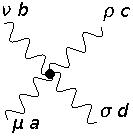
\includegraphics[scale=0.3]{Vert_A4.jpg}
 \end{center}
\end{minipage}

\begin{minipage}[c]{0.45\linewidth}
 \begin{equation*}
  V_{A^3} = -igf^{abd} \Big[ (p-k)_{\rho} g_{\mu \nu} + (k-q)_{\mu} g_{\nu \rho} + (q-p)_{\nu} g_{\mu \rho} \Big]
 \end{equation*}
\end{minipage} \hfill
\begin{minipage}[c]{0.45\linewidth}
 \begin{center}
%  \includegraphics[scale=0.3]{Vert_A3.jpg}
 \end{center}
\end{minipage}

\begin{minipage}[c]{0.45\linewidth}
 \begin{equation*}
  V_{\bar{C} C A} = -igf^{abd} (k-q)_{\mu} 
 \end{equation*}
\end{minipage} \hfill
\begin{minipage}[c]{0.45\linewidth}
 \begin{center}
%  \includegraphics[scale=0.3]{Vert_CCA.jpg}
 \end{center}
\end{minipage}\\

\noindent
We are computing the two tadpoles with a vertice having three branches. We start by computing the tadpole with a loop of ghost.
\begin{eqnarray*}
 \Gamma_{\bar{C} C A} &=& \int \frac{d^4k}{(2 \pi)^4} \left(\frac{-ig}{2}\right) f^{abd} 2 k_{\mu} \frac{- \delta^{ab}}{k^2+i0} \\
                          &=& \delta^{ab}  \Bigg( igf^{abd} \int \frac{d^4k}{(2 \pi)^4} \frac{ k_{\mu} }{ k^2+i0 }  \Bigg)
\end{eqnarray*}

\noindent
Now we compute the tadpole with a loop of gauge field.
\begin{eqnarray*}
 \Gamma_{A^3} (k) &=& \int \frac{d^4k}{(2 \pi)^4} (-ig) f^{abc} \Big[ (p-k)_{\rho} g_{\mu \nu} + 2k_{\mu} g_{\mu \rho} - (k+p)_{\nu} g_{\mu \rho} \Big] \frac{-\delta^{bc} g_{\nu \rho}}{k^2 + i0} \\
                  &=& \delta^{bc} \Bigg( igf^{abc} \int \frac{d^4k}{(2 \pi)^4} \Big[ (p-k)_{\nu} g_{\mu \nu} + 2k_{\mu} g_{\mu \nu} - (k+p)_{\nu} g_{\mu \nu} \Big] \frac{1}{k^2 + i0} \Bigg) \\
                  &=& \delta^{bc} \Bigg( 2igf^{abc} \int \frac{d^4k}{(2 \pi)^4} \frac{k_{\mu} g_{\nu \nu} - k_{\nu} g_{\mu \nu}}{k^2 + i0} \Bigg) \\
                  &=& \delta^{bc} \Bigg( 2igf^{abc} \int \frac{d^4k}{(2 \pi)^4} \frac{4 k_{\mu} - k_{\nu} g_{\mu \nu}}{k^2 + i0} \Bigg) \\
                  &=& \delta^{bc} \Bigg( 6igf^{abc} \int \frac{d^4k}{(2 \pi)^4} \frac{k_{\mu}}{k^2 + i0} \Bigg)
\end{eqnarray*}
Our goal was there to see of these two tadpole cancel even when we factorize by $\delta^{ab}$. The conclusion is that there is not such cancellation as we hoped to have.

\subsection*{BRST Symetry (Becchi, Rouet, Stora, et Tyupkin)}

\noindent
When we wrote $\mathcal{S}$, we had to fixe the gauge, in fact without doing this the integral that we obtain diverge. We noticed previoulsy that the pure Yang-mills Lagrangian is invariant under the gauge transformation. However we are not working anymore with this pure Lgrangian, we added new terms which destroy this invariance. It seems that we don't have any invaraince now, but C. Becchi, A. Rouet, R. Stora, et I. V. Tyupkin discovered a new symetry. This symetry is in fact a particular gauge transformation. To define this new symetry, that we will call now BRST symetry, we need to re-define the gauge parameter, that we had in our previously gauge transformation \big($ A^{\omega}_{\mu} \simeq A_{\mu} - [A_{\mu},u] + \partial_{\mu}u + \mathcal{O} (u)$\big). \\
We set $ u = c$., where $c$ is a grasmman vrariable. To do this modification will change nothing to that fact that the pure part is gauge invariant. 

\noindent
\begin{eqnarray}
 A^{\omega \hspace{1mm} a}_{\mu}    &\simeq&    A^{a}_{\mu} - f^{abd} A^{a}_{\mu} c^{a} + \partial_{\mu}c^{a}  + \mathcal{O} (c^{a})\\
                                    &\simeq&    A^{a}_{\mu}  + D_{\mu} c^{a} + \mathcal{O} (c^{a})
\end{eqnarray}
\begin{eqnarray}
 \partial_{\mu}  A^{\omega \hspace{1mm} a}_{k}    &\simeq&    \partial_{\mu} A^{a}_{k} - f^{abd}  \partial_{\mu} \left( A^{a}_{k} c^{a} \right) 
+ \Box c^{a} + \mathcal{O} (c^{a})  \\
                                                  &\simeq&     \partial_{\mu} A^{a}_{k}  + \partial_{\mu}D_{\mu} c^{a} + \mathcal{O} (c^{a})
\end{eqnarray}
\begin{eqnarray}
 \left( \partial_{\mu}  A^{\omega \hspace{1mm} a}_{k} \right)^{2} &\simeq&  \left( \partial_{\mu} A^{a}_{k} \right)^{2} 
+ 2 \left(  \partial_{\mu}D_{\mu} c^{a}  \right) \left( \partial_{\mu} A^{a}_{k} \right) + \mathcal{O} (c^{a})  
\end{eqnarray}

\begin{eqnarray}
 \mathcal{L}_{fix.}  \rightarrow \frac{1}{2 \alpha} \left( \partial_{\mu} A^{a}_{k} \right)^{2} 
+ \frac{1}{\alpha} \left(  \partial_{\mu}D_{\mu} c^{a}  \right) \left( \partial_{\mu} A^{a}_{k} \right) + \mathcal{O} (c^{a})  
\end{eqnarray}

\begin{eqnarray}
 \mathcal{L}_{FP} &=&  \overline{c}^{a} \left( \Box c^{a} -g f^{abd} \partial_{\mu} \left( A^{b}_{\mu} c^{d} \right) \right) \\
                  &=&  \overline{c}^{a} M  c^{a}
\end{eqnarray}

\begin{eqnarray}
 \overline{c}^{a} &\rightarrow& \overline{c}^{a} - \frac{1}{\alpha} \left( \partial_{\mu} A^{a}_{\mu} \right) ,
\end{eqnarray}

\begin{eqnarray}
 D_{\mu}c^{a}  \rightarrow  D_{\mu}c^{a} &+& f^{abd} f^{ben} A^{e}_{\mu} c^{n} c^{d}  +  f^{abd} \left(  \partial_{\mu} c^{b} \right) c^{d}  
\end{eqnarray}

\begin{eqnarray}
 D_{\mu}c^{a}  \rightarrow  D_{\mu}c^{a} &+& f^{abd} f^{ben} A^{e}_{\mu} c^{n} c^{d}  
+  \frac{1}{2} f^{abd} f^{den} A^{b}_{\mu} c^{e} c^{n}  \nonumber \\
                                         &+& f^{abd} \left(  \partial_{\mu} c^{b} \right) c^{d}  
- \frac{1}{2}  f^{abd}  \left( \partial_{\mu} c^{b} c^{d} \right)  
\end{eqnarray}

\begin{eqnarray}
 f^{abd} f^{ben} c^{n} c^{d}  = \frac{1}{2} f^{abd} f^{den} c^{e} c^{n}
\end{eqnarray}

\begin{eqnarray}
 A^{a}_{\mu}    &\rightarrow&    A^{a}_{\mu} - f^{abd} A^{a}_{\mu} c^{a} + \partial_{\mu}c^{a} \\
 \overline{c}^{a} &\rightarrow& \overline{c}^{a} - \frac{1}{\alpha} \left( \partial_{\mu} A^{a}_{\mu} \right) \\
c^{a} &\rightarrow& c^{a} - \frac{1}{2} f^{abd} c^{b} c^{d}
\end{eqnarray}

\begin{equation}
J= \left(
 \begin{array}{lcr}
    \delta_{\mu \nu} \delta^{ab}                     & D_{\mu} \delta^{ab}              & 0   \\
    0                                                & \delta^{ab} - f^{adb} c^{d}      & 0   \\
    \delta^{ab} \frac{1}{\alpha}\partial_{\mu}       & 0                                 &\delta^{ab}  
 \end{array} \right).
\end{equation}

\begin{eqnarray}
 det \left( J \right) = 1.
\end{eqnarray}

\section{The noncommutative space $\mathbb{R}^{3}_{\lambda}$}

\subsection*{Product on $\mathbb{R}^{3}_{\lambda}$}

\noindent
We consider first $\mathbb{R}^{4}$, which can be viewed as $\mathbb{C}^{2}$. Then we choose to work with $S^3_\rho$, the 3-sphere of radius $\rho$.




\noindent
The 3-sphere which is living in $\mathbb{R}^{4}$ can be interpreted as the Hopf fibration.
\begin{dfn}
 The standart 3-sphere is the set of points $(x_1,x_2,x_3,x_4)$ in $\mathbb{R}^{n+1}$ that satisfy the equation,
 \begin{equation*}
  x_1^2 + x_2^2 + x_3^2 + x_4^2 = \rho^2.
 \end{equation*}
\end{dfn}




We are going to consider $\mathbb{R}^{3}_{\lambda}$ a deformation of $\mathbb{R}^{3}$, the reason to consider a deformation of this euclidean space is because our goal is to build a quantum system of which the classical system is the "shadow". And to do this one approach is to deform the pointwise product on the algebra of functions on the phase space into a family of noncommutative products.\\ The noncommutative space $\mathbb{R}^{3}_{\lambda}$ is an associative $*$-algebra with unit $\mathbb{I}$ and center\footnote{The center of an algebra consists of the elements of the algebra wich commute with every elements of this algebra.} $\mathcal{Z}(\mathbb{R}^{3}_{\lambda})$. Let's recall the definition of a $*$-algebra.
\dfn{
A $*$-algebra is a set $\mathbb{A}$ of bounded linear operators \footnote{Any mapping between two vector space is called an operator.} on a Hilbert space which satified the three following conditions, 
 \begin{equation*}
  c A + d B \in \mathbb{A}, \hspace{1cm}  A B \in \mathbb{A}, \hspace{1cm} A^{*} \in \mathbb{A},
 \end{equation*}
$\forall$ $A$, $B$ $\in$ $\mathbb{A}$, and $c$, $d$ $\in$ $\mathbb{C}$.
}\\

\noindent
We refresh our memory by recalling the definition of a Hibert space and a bounded operator.
\dfn{
A Hilbert space $H$ is a vector space endowed with an inner product and associated norm and metric, such that every Cauchy sequence in $H$ has a limit in $H$.
}
\dfn{
Let $X$, $Y$ be two normed vector spaces and $T:X \rightarrow Y$ a linear operator. We say that $T$ is bounded if there exists a number $c \leq 0$ such that
\begin{equation*}
 \| T x \|_{Y} \leq \| x \|_{X}
\end{equation*}
for all $x$ $\in$ $X$.
}\\

\noindent
From an other view point, $\mathbb{R}^{3}_{\lambda}$ can be viewed as a particular subalgebra of $\mathbb{R}^{4}_{\theta}$, which is the associative algebra of functions on $\mathbb{R}^4$ endowed with the Wick-Voros product. 
\begin{equation*}
 \phi\star \psi\, (z_a,\bar z_a)= \phi(z,\bar z) \exp(\theta \overleftarrow \partial_{z_a}\overrightarrow \partial_{\bar z_a}) \psi(z,\bar z), \,\,\,\, a=1,2 \label{Wick-Vorosprod}
\end{equation*}
For coordinate functions we have,
\begin{eqnarray*}
 z_a \star \bar{z_b} &=& z_a \exp(\theta \overleftarrow \partial_{z_d}\overrightarrow \partial_{\bar z_d}) \bar{z}_{b} \\
                     &=& \theta \delta_{ad} \delta_{bd} \\
                     &=& \theta \delta_{ab} \\
 \bar{z_b} \star z_a &=& \bar{z}_{b} \exp(\theta \overleftarrow \partial_{z_d}\overrightarrow \partial_{\bar z_d}) z_a \\
                     &=& 0.
\end{eqnarray*}
Thus,
\begin{equation*}
 [z_a,\bar z_b]_\star= \theta \delta_{ab} 
\end{equation*}
with $\theta$ a constant, real parameter.\\

\noindent
The crucial step  to obtain star products on the space of function on $\mathbb{R}^3$, hence to deform this algebra into a noncommutative algebra, is to identify $\mathbb{R}^3$ with the dual, $\mathfrak{g}^*$,  of some chosen three dimensional Lie algebra $\mathfrak{g}$. We choose here to work with the $\mathfrak{su}(2)$ Lie algebra.
\begin{dfn}
A Lie Algebra $\mathfrak{g}$ (finite dimensional or not) over $\mathbb{R}$ or $\mathbb{C}$ is a vetor space equipped with a Lie bracket, i.e. a bilinear maps,
\begin{equation*}
 \left\{ 
  \begin{array}{rcl}
   \mathfrak{g} \times \mathfrak{g} & \rightarrow & \mathfrak{g} \\ 
   (X,Y) & \rightarrow & \big[X,Y\big]
  \end{array}
 \right.
\end{equation*}
wich is antisymetric, i.e. $\big[X,Y\big] = - \big[Y,X\big]$, and fullfill antisymetric and the Jacoby identity, i.e. $\Big[X,\big[Y,Z\big]\Big] + \Big[Y,\big[Z,X\big]\Big] + \Big[Z,\big[X,Y\big]\Big]$.\\
\end{dfn}

\noindent
The standard mathematical representation of the lie algebra $\mathfrak{su}(2)$ consists of the traceless antihermitian $2 \times 2$ complex matrices, with the regular commutator as Lie bracket. A direct calculation show that the Lie algebra $\mathfrak{su}(2)$ is the 3-diemensional real algebra spanned by the set $\{ i \sigma_{j} \}$.
\begin{equation*}
 \mathfrak{su}(2) = span \{ i \sigma_{1} , i \sigma_{2} , i \sigma_{3} \} ,
\end{equation*}
where the $\sigma_i$ $(i=1,2,3)$ are the Pauli matrices,
\begin{equation*}
 \sigma_{1} = 
  \begin{pmatrix}
    0 & 1 \\
    1 & 0 
   \end{pmatrix}, \quad
 \sigma_{2} = 
  \begin{pmatrix}
    0 & i \\
    i & 0 
   \end{pmatrix}, \quad
 \sigma_{3} = 
  \begin{pmatrix}
    1 & 0 \\
    0 & -1 
   \end{pmatrix}. 
\end{equation*}

\noindent
The fact to consider $\mathfrak{su}(2)$ as "our" lie algebra induce,
\begin{equation}
 \{ x_i , x_j \} = f_{ijk} x_k, \label{bracket_su(2)}
\end{equation}
with $i=1, 2, 3$, and $f_{ijk}$ the structure constant of $\mathfrak{su}(2)$. But we can show that $\mathfrak{su}(2)$ is a subalgebra of $\mathfrak{sp}(4)$, which can be viewed as the poisson algebra on quadratic function on $\mathbb{R}^4$ with canonical Poisson bracket,
\begin{equation*}
 \{ z_a , \bar{z}_b \} = i.
\end{equation*}
Indeed it is possible to find quadratic functions
\begin{equation*}
 \pi^*(x_i)= \pi^*(x_i)(z^a,\bar z^a)
\end{equation*}
which obey \ref{bracket_su(2)}.We have indicated with $\pi^*$ the  pull-back map $\pi^*:\mathcal{F}(\mathbb{R}^3)\rightarrow \mathcal{F}(\mathbb{R}^4)$. Then one can show  that this Poisson subalgebra is also a Wick-Voros  subalgebra, that is
\begin{equation*}
 \pi^*(x_i)(z^a,\bar z^a)\star \pi^*(x_j)(z^a,\bar z^a) -\pi^*(x_j)(z^a,\bar z^a)\star \pi^*(x_i)(z^a,\bar
z^a)= \lambda c_{ij}^k \pi^*(x_k)(z^a,\bar z^a)
\end{equation*}
where the noncommutative parameter $\lambda$  shall be adjusted according to  the physical dimension of the coordinate functions $x_i$. Here we will consider quadratic realizations of the kind
\begin{equation*}
 \pi^*(x_\mu)=\frac{\lambda}{\theta} \bar z^a e_\mu^{ab} z^b, \;\;\; \mu=0, ..,3 \label{xmu}
\end{equation*}
with $\lambda$ a constant, real parameter of length dimension equal to one, $e_i= \frac{1}{2}\sigma_i, \: i=1,..,3$ are the $SU(2)$ generators in the defining representation with  $\sigma_i$
the Pauli matrices, while $e_0=\frac{1}{2} \mathbf{1}$.  We  shall omit the pull-back map from now, unless necessary. Notice that
\begin{equation*}
x_0=\frac{\lambda}{2\theta}\bar z_a z_a
\end{equation*}
commutes with $x_i$ so that we can alternatively define $\mathbb{R}^3_\lambda$ as the commutant of $x_0$; $x_0$ generates the center of the algebra. We also have
\begin{equation*}
 x_0^2= \sum_i x_i^2.
\end{equation*}
We can show that the induced $\star$-product reads,
\begin{equation*}
 \phi \star \psi (x) = exp \left[ \frac{\lambda}{2} ( \delta_{ij} x_0 + i \epsilon_{ijk} x_k ) \frac{\partial}{\partial u_i} \frac{\partial}{\partial v_j} \right] \phi(u) \psi(v) |_{u=v=x}
\end{equation*}
for any $\phi$, $\psi$ $\in$ $\mathbb{R}^{3}_{\lambda}$, implies:
\begin{eqnarray*}
 && x_i \star x_j = x_i x_j + \frac{\lambda}{2} ( \delta_{ij} x_0 + i \epsilon_{ijk} x_k ),\\
 && x_0 \star x_i = x_i \star x_0 = x_0 x_i + \frac{\lambda}{2} x_i  ,\\
 && x_0 \star x_0 = x_{0}^{*2} = x_0 ( x_0 + \frac{\lambda}{2} ) = \sum_{i=1}^{3} x_i \star x_i - \lambda x_0,
\end{eqnarray*}
from wich we obtain
\begin{equation*}
 [x_i , x_j ]_{\star} = i \lambda \epsilon_{ijk} x_{k}.
\end{equation*}
We have thus realized the announced isomorphism between the algebra of linear functions on $\mathbb{R}^3\simeq \mathfrak{su}(2)^*$ endowed with the $\star$ commutator and the $\mathfrak{su}(2)$ Lie algebra. Thus, the algebra $\mathbb{R}^3_\lambda$ can be defined as $\mathbb{R}^3_\lambda=\mathbb{C}[x_\mu]/{\cal{I}}_{{\cal{R}}_1,{\cal{R}}_2 }$, i.e the quotient of the free algebra generated by the coordinate functions $(x_i)_{i=1,2,3}, x_0,$ by the two-sided ideal generated by the relation ${\cal{R}}_1: [x_i,x_j]_\star=i\lambda\epsilon_{ijk}x_k$, together with ${\cal{R}}_2: x_0\star x_0 +\lambda x_0 =\sum_i x_i\star x_i$. Notice that, because of the presence of $x_0$ $\mathbb{R}^3_{\lambda\ne 0}$ {\it is not} isomorphic to  $ {\cal{U}}(\mathfrak{su}(2))$.

\section{The matrix basis}

[blablabla]

\section{The classical gauge action $\mathbb{R}^{3}_{\lambda}$}

\subsection*{General properties on differential calculus}

\noindent
Let $\mathbb{A}$ be an associative $*$-algebra with unit $\mathbb{I}$ and center $\mathcal{Z}(\mathbb{A})$. We denote the involution by $a \rightarrow a^{\dagger}$, $\forall$ $a$ $\in$ $\mathbb{A}$. Here, basically, the role of the vector fields is now played by the derivations of the algebra. 

\begin{dfn}
The vector space of derivations of $\mathbb{A}$ is the space of linear maps defined by $ Der(\mathbb{A}) = \{ X : \mathbb{A} \rightarrow \mathbb{A} | X(ab) = X(a)b + aX(b), \forall a, b \in \mathbb{A} \}.$
The derivation $X$ $\in$ $Der(\mathbb{A})$ is called real if $\Big( X(a) \Big)^{\dagger} = X(a^{\dagger})$, $\forall a \in \mathbb{A}$.
\end{dfn}

\begin{prop}
 $ Der(\mathbb{A}) $ is a $\mathcal{Z}(\mathbb{A})$-module for the product $(fX)a = f(Xa)$, $\forall f \in \mathcal{Z}(\mathbb{A})$, $\forall X \in Der(\mathbb{A})$ and a Lie algebra for the bracket $[X,Y]a = XYa - YXa, \forall X, Y \in Der(\mathbb{A}) $ is a $\mathcal{Z}(\mathbb{A})$.
\end{prop}

\noindent
The main features of the differential calculus based on $Der(\mathbb{A})$ are involved in the following proposition. Notice that both the Lie algebra structure and the $\mathcal{Z}(A)$-module structures for $Der(\mathcal{A})$ are used as essential ingredients in the construction.
\begin{prop}
 Let $\Omega^{n}_{Der}(\mathcal{A})$ denote the space of $\mathcal{Z}(\mathbb{A})$ multilinear linear antisymetric maps from $Der(\mathbb{A})^{n}$ to $\mathbb{A}$, with $\Omega^{0}_{Der}(\mathcal{A})=\mathbb{A}$ and let $\Omega^{\bullet}_{Der}(\mathbb{A}) = \bigoplus_{n \geq 0} \Omega^{n}_{Der}(\mathcal{A})$. Then $\left( \Omega^{\bullet}_{Der}(\mathbb{A}) = \bigoplus_{n \geq 0} \Omega^{n}_{Der}(\mathcal{A}),\times, d \right)$
 $\forall X, Y \in Der(\mathbb{R}^{3}_{\lambda})$ , $\forall a \in \mathbb{R}^{3}_{\lambda}$, which is also a module over $\mathcal{\mathbb{A}}$. Any Lie subalgebra $\mathcal{G}$ of $Der(\mathbb{R}^{3}_{\lambda})$, which is still a module over $\mathcal{Z}(\mathbb{R}^{3}_{\lambda})$ generates a differential calculus, with $\mathbb{N}$-graded differential algebra $\left( \Omega^{\bullet}_{\mathcal{G}}(\mathbb{A}) = \bigoplus_{n \geq 0} \Omega^{n}_{\mathcal{G}}(\mathcal{A}),\times, d \right)$, where:
\begin{description}
 \item $\Omega^{n}_{\mathcal{G}}(\mathcal{A})$ is the space of $\mathcal{Z}(\mathbb{A})$-n-linear antisymetric maps $\omega : \mathcal{G}^{n} \rightarrow \mathbb{A}$,
 \item $\times$ is the inner product over $\Omega^{\bullet}_{\mathcal{G}}(\mathbb{A})$,
 \item and $d : \Omega^{n}_{\mathcal{G}}(\mathcal{A}) \rightarrow \Omega^{n+1}_{\mathcal{G}}(\mathcal{A})$ is the nilpotent differential. 
\end{description}
\end{prop}



\subsection*{Application for $\mathbb{R}^{3}_{\lambda}$}

\noindent
Let $Der(\mathbb{R}^{3}_{\lambda})$ be the Lie algebra of real derivations of $\mathbb{R}^{3}_{\lambda}$ defined by 
\begin{equation*}
 \left[ D_i , D_j \right]a = ( D_i D_j - D_j D_i )a, 
\end{equation*}
$\forall X, Y \in Der(\mathbb{R}^{3}_{\lambda})$ , $\forall a \in \mathbb{R}^{3}_{\lambda}$, which is also a module over $\mathcal{\mathbb{A}}$. Any Lie subalgebra $\mathcal{G}$ of $Der(\mathbb{R}^{3}_{\lambda})$, which is still a module over $\mathcal{Z}(\mathbb{R}^{3}_{\lambda})$ generates a differential calculus, with $\mathbb{N}$-graded differential algebra $\left( \Omega^{\bullet}_{\mathcal{G}}(\mathbb{A}) = \bigoplus_{n \geq 0} \Omega^{n}_{\mathcal{G}}(\mathcal{A}),\times, d \right)$, where:
\begin{description}
 \item $\Omega^{n}_{\mathcal{G}}(\mathcal{A})$ is the space of $\mathcal{Z}(\mathbb{A})$-n-linear antisymetric maps $\omega : \mathcal{G}^{n} \rightarrow \mathbb{A}$,
 \item $\times$ is the inner product over $\Omega^{\bullet}_{\mathcal{G}}(\mathbb{A})$,
 \item and $d : \Omega^{n}_{\mathcal{G}}(\mathcal{A}) \rightarrow \Omega^{n+1}_{\mathcal{G}}(\mathcal{A})$ is the nilpotent differential. 
\end{description}

\noindent
We consider now the simple differential calculus generated by the Lie algebra of real inner derivations of $\mathbb{R}^{3}_{\lambda}$ defined by
\begin{equation*}
 \mathcal{G} = \{ D_i = \frac{i}{\kappa^2} [ x_i , . ] , i=1,2,3 \},
\end{equation*}
with the relation
\begin{equation*}
 \left[ D_i , D_j \right] = \frac{-\lambda}{\kappa^2} D_k , \hspace{5mm} \forall i,j,k =1,2,3.
\end{equation*}

\noindent
We further assume that the algebra $\mathbb{R}^{3}_{\lambda}$ plays the role of a right-module on itself. Thus a connection on $\mathbb{R}^{3}_{\lambda}$ can be defined as a linear map $\nabla_{D_i} := \nabla_{D_i} : \mathbb{R}^{3}_{\lambda} \rightarrow \mathbb{R}^{3}_{\lambda}$ satisfying
\begin{eqnarray*}
 && \nabla_{i} (ma) = m D_i (a) + \nabla_i (m) a \\
 && \nabla_{ f D_i } = \nabla_i (m) f \\
 && \nabla_{ D_i + D_j } = \nabla_{i}(m) + \nabla_{j} (m)
\end{eqnarray*}
for any $D_i , D_j \in \mathcal{G}$, $a \in \mathbb{R}^{3}_{\lambda}$, $m \in \mathbb{R}^{3}_{\lambda}$, and $f \in \mathcal{Z}(\mathbb{R}^{3}_{\lambda})$. The hermitean connections, used here, satisfy for any real derivation $D$ in $\mathcal{G}$
\begin{equation*}
 D( h(a_1 ,a_2 ) ) = h \left( \nabla_{D}(a_1) , a_2 \right) + h \left( a_1 , \nabla_{D}(a_2) \right), \hspace{5mm} \forall m_1 , m_2 \in \mathbb{M}, 
\end{equation*}
where $h(a_1 , a_2 ) = a_{1}^{\dagger} a_{2}$, $\forall a_1 , a_2 \in \mathbb{R}^3_{\lambda}$, denotes the hermitean structure. The curvature is the linear map $F( D_i , D_j ) : \mathbb{R}^3_{\lambda} \rightarrow \mathbb{R}^3_{\lambda} $ defined by 
\begin{equation*}
 F( D_i , D_j )m = \left[ \nabla_X , \nabla_Y \right]m - \nabla_{[X,Y]}m, \hspace{5mm} \forall X,Y \in \mathcal{G}. 
\end{equation*}
In our case where we assume that $\mathbb{R}^{3}_{\lambda}$ plays the role of a right-module on itself, a hermitean connection is entirely determined by $\nabla_{D}(\mathbb{I})$, with $\nabla_{D}(\mathbb{I})^{\dagger} = - \nabla_{D}(\mathbb{I})$.

\noindent
We have the following curvature:
\begin{equation*}
 F_{ij} = - i ( D_{i} A_{j}  -  D_{j} A_{i} ) - [ A_{i} , A_{j} ] - \frac{i \lambda }{\kappa^{2}} \epsilon_{ijk} A_{k}. 
\end{equation*}
We set $ \Phi_{ij} = - i ( D_{i} A_{j}  -  D_{j} A_{i} ) - [ A_{i} , A_{j} ] $ and consider the simplest analog of a Yang-Mills action, given by:
\begin{eqnarray*}
 S_{cl} &=& Tr(F_{ij}^{\dagger} F_{ij}) \\
        &=& Tr(-\Phi_{ij}\Phi_{ij}+i\frac{2\lambda}{\kappa^2}\epsilon_{ijk}\Phi_{ij}A_{k}+\frac{2\lambda^2}{\kappa^4}A_iA_i)
\end{eqnarray*}
As gauge, we choose $D_{i} A_{i}=0$. The action gauge fixed can be written in the following way:
\begin{equation*}
 S_{cl,gf} = Tr \Bigg[ - \Phi_{ij}\Phi_{ij}+i\frac{2\lambda}{\kappa^2}\epsilon_{ijk}\Phi_{ij}A_{k}+\frac{2\lambda^2}{\kappa^4}A_iA_i + \frac{1}{2\xi}(D_iA_i)^2 + \bar{c} \left( D^2 +D_i [A_i , c] \right) \Bigg]. 
\end{equation*}
If we stop now, we will have a kinetic operator for the gauge field non diagonal, which is a problem, because we don't know how to inverse a such operator. But we know how to inverse a diagonal one, thus the idea is to add terms in such a way to have a diagonal operator.

\subsection*{Actions}

\noindent
The action that we consider is,
\begin{equation*}
 S = S_{cl} + S_{GF} + S_{add},
\end{equation*}
with
\begin{eqnarray*}
 S_{cl}    &=&   Tr \Bigg[-F_{\mu \nu} F_{\mu \nu}+\frac{2 i \lambda}{\kappa^2}\epsilon_{\mu \nu \rho}\Phi_{\mu \nu}A_{\rho}+\frac{2\lambda^2}{\kappa^4}A_\mu A_\mu \Bigg], \\
 S_{GF} &=&   s Tr \Bigg[ \bar{c} (D_\mu A_\mu) + \alpha \bar{c} b \big) \Bigg], \\
 S_{add}    &=&   Tr \Bigg[ \gamma \epsilon_{\mu \nu \rho} \mathcal{A}_\mu F_{\nu \rho} + \Delta \epsilon_{\mu \nu \rho} \mathcal{A}_{\mu} \mathcal{A}_{\nu} \mathcal{A}_{\rho} \Bigg].
\end{eqnarray*}

\subsection*{Useful relations}

\noindent
We summarize below some useful relations for the computaions that we will have to do.
\begin{eqnarray*}
 && \epsilon_{\mu \nu \rho} \epsilon_{\alpha \nu \rho} = 2 \delta_{\mu \alpha}, \\
 && D_\mu A_\nu = \eta_\mu A_\nu - A_\nu \eta_\mu ,\\
 && \big[ \eta_\mu , \eta_\nu \big] = - \frac{\lambda}{\kappa^2} \epsilon_{\mu \nu \rho} \eta_\rho ,\\
 && \epsilon_{\mu \nu \rho} \eta_\mu \eta_\nu A_\rho = - \frac{\lambda}{\kappa^2} \delta_{\mu \nu} \eta_\mu A_\nu ,\\
 && \big[ D_\mu , D_\nu \big] = D_\mu D_\nu - D_\nu D_\mu = - \frac{\lambda}{\kappa^2} \epsilon_{\mu \nu \rho} D_\rho ,\\
 && s A_\mu = D_\mu c - i [A_\mu,c] = [ \mathcal{A}_\mu , c] ,\\
 && sc = icc ,\\
 && s\bar{c} = b ,\\
 && sb = 0 .
\end{eqnarray*}

\subsection*{Simplest analog of the Yang-Mills action - Classical part}

\begin{eqnarray*}
 S_{cl} &=& Tr \Big[ -F_{\mu \nu} F_{\mu \nu}+i\frac{2\lambda}{\kappa^2} \epsilon_{\mu \nu \rho} F_{\mu \nu} A_{\rho} + \frac{2\lambda^2}{\kappa^4} \delta_{\mu \nu} A_\mu A_\nu \Big]
\end{eqnarray*}
   
\begin{eqnarray*}
 F_{\mu \nu} F_{\mu \nu} &=& \Bigg( - i \Big( D_{\mu} A_{\nu}  -  D_{\nu} A_{\mu} \Big) - \Big[A_{\mu},A_{\nu} \Big] \Bigg) . \Bigg( - i \Big( D_{\mu} A_{\nu}  -  D_{\nu} A_{\mu} \Big) - \Big[A_{\mu},A_{\nu}\Big] \Bigg) \\
                         &=& A_\mu \Big( 2 \delta_{\mu \nu} D^2 - 2 D_\nu D_\mu \Big) A_\nu - 4i A_\mu A_\nu (D_\mu A_\nu) + 4i A_\mu A_\nu (D_\nu A_\nu) + 2 A_\mu A_\nu A_\mu A_\nu - 2 A^4
\end{eqnarray*}

\begin{eqnarray*}
 \epsilon_{ijk} F_{ij} A_k &=& \epsilon_{ijk} \left( - i ( D_{i} A_{j}  -  D_{j} A_{i} ) - [ A_{i} , A_{j} ] \right) A_k \\
                              &=& A_i \left[ 2 i \epsilon_{ijk}  D_k \right] A_j - 2 \epsilon_{ijk} A_i A_j A_k 
\end{eqnarray*}

\begin{eqnarray*}
 S_{cl} &=& Tr \Big[ A_i \left( - 2 \delta_{ij} D^2 + 2 D_j D_i - \frac{4\lambda}{\kappa^2} \epsilon_{ijk}  D_k + \frac{2\lambda^2}{\kappa^4} \delta_{ij} \right) A_j \\
     && \hspace{1cm} + 2 A^4 -2 A_i A_j A_i A_j + 8i A_i A_j A_i \eta_j - 4i A_i A^2 \eta_i - 4i A^2 A_i \eta_i - \frac{4i\lambda}{\kappa^2} \epsilon_{ijk} A_i A_j A_k  \Big]
\end{eqnarray*}

\subsection*{Gauge fixing} 

\noindent
A BRST-invariant gauge-fixed action can be written as:
\begin{equation*}
 S = S_0 + S_1 + S_{GF} 
\end{equation*}
where $\alpha$ is a real gauge parameter and $s$ is a nipoltent Slavnov operation. $\bar{c}$, $c$, $b$ are respectively the antighost, ghost, and Stueckelberg field with rescpective ghost number $-1$, $+1$, and $0$. Recall that $s$ acts as graded derivation with respect to the grading defined by the sum of the degree of forms and ghost number (modulo 2), by using the properties of the action of $s$ on the different fields, and integrating over the Stueckelberg field, we obtain:
\begin{equation*}
 S = S_0 + S_1 + Tr \left[ \frac{-1}{4 \alpha} (D_i A_i)^2 - \bar{c} \big( D^2 c - i D_i [A_i , c] \big) \right]
\end{equation*}
Thus:
\begin{eqnarray*}
 S_{GF} &=& Tr \left[ \frac{-1}{4 \alpha} (D_i A_i)^2 - \bar{c} \big( D^2 c - i D_i [A_i , c] \big) \right] \\
        &=& Tr \left[ A_i \big[ \frac{1}{4 \alpha} D_i D_j \big] A_j - \bar{c} \big( D^2 c - i D_i [A_i , c] \big) \right]
\end{eqnarray*}

\subsection*{Additional terms}

\begin{equation*}
 S_{add} = Tr \Bigg[ \gamma \epsilon_{ijk} \mathcal{A}_i \Phi_{jk} + \Delta \epsilon_{ijk} \mathcal{A}_{i} \mathcal{A}_{j} \mathcal{A}_{k} \Bigg]
\end{equation*}

\begin{eqnarray*}
 \gamma \epsilon_{\mu \nu \rho} \mathcal{A}_\mu F_{\nu \rho} 
                 &=& \gamma \epsilon_{\mu \nu \rho} \Big( -i A_\mu + \eta_\mu \Big) \Bigg( - i \big(D_{\nu} A_{\rho}-D_{\rho} A_{\nu}\big) - [A_{\nu},A_{\rho}] - \frac{i \lambda}{\kappa^{2}} \epsilon_{\nu \rho \alpha} A_{\alpha} \Bigg) \\            
\end{eqnarray*}

\begin{eqnarray*}
 \Delta \epsilon_{ijk} \mathcal{A}_{i} \mathcal{A}_{j} \mathcal{A}_{k} &=& \Delta \epsilon_{ijk} ( -i A_i + \eta_i ) ( -i A_j + \eta_j ) ( -i A_k + \eta_k ) \\
                       &=& \Delta \epsilon_{ijk} \left( i A_i A_j A_k - A_i A_j \eta_k - A_i \eta_j A_k - i A_i \eta_j \eta_k \right. \\
                       && \left. - \eta_i A_j A_k - i \eta_i A_j \eta_k - i \eta_i \eta_j A_k +  \eta_i \eta_j \eta_k  \right) \\
                       &=& \Delta \epsilon_{ijk} \left( i A_i A_j A_k + \eta_i \eta_j \eta_k  + 3 A_i \eta_k A_j - 3 i \eta_i \eta_j A_k \right) \\
                       &=& A_i \big[ 3 \Delta \epsilon_{ijk} \eta_k \big] A_j + i \Delta \epsilon_{ijk} A_i A_j A_k + \Delta \epsilon_{ijk} \eta_{i} \eta_j \eta_k - 3i \Delta \epsilon_{ijk} \eta_i \eta_j A_k
\end{eqnarray*}

\begin{eqnarray*}
 S_{add} &=& Tr \Big[ A_i \Big[ 2 \gamma \epsilon_{ijk} D_k - \frac{2 \gamma \lambda}{\kappa^{2}} \delta_{ij} + 2 \gamma \epsilon_{ijk} \eta_{k} + 3 \Delta \epsilon_{ijk} \eta_k \Big] A_j \\ 
     && \hspace{1cm} + ( 2 \gamma + \Delta ) i \epsilon_{ijk} A_i A_j A_k - ( 4 \gamma + 3 \Delta ) i \epsilon_{ijk} \eta_i \eta_j A_k - \frac{2i \gamma \lambda}{\kappa^2} \delta_{ij} \eta_i A_j + \Delta \epsilon_{ijk} \eta_{i} \eta_j \eta_k \Big]
\end{eqnarray*}



\subsection*{Full action}

\begin{eqnarray*}
 S &=& S_0 + S_g + S_1 \\
   &=& Tr\Bigg[ A_i \Bigg( - 2 \delta_{ij} D^2 + 2 D_j D_i - \frac{4\lambda}{\kappa^2} \epsilon_{ijk}  D_k + \frac{2\lambda^2}{\kappa^4} \delta_{ij} \Bigg) A_j \\
   && \hspace{15mm} + 2 A^4 -2 A_i A_j A_i A_j + 8i A_i A_j A_i \eta_j - 4i A_i A^2 \eta_i - 4i A^2 A_i \eta_i - \frac{4i\lambda}{\kappa^2} \epsilon_{ijk} A_i A_j A_k \\
   && \hspace{1cm} + A_i \Bigg( - \frac{1}{4 \alpha} D_i D_j \Bigg) A_j + \bar{c} \big( D^2 c +D_i [A_i , c] \big) \\
   && \hspace{1cm} + A_i \Bigg( 2 \gamma \epsilon_{ijk} D_k - \frac{2 \gamma \lambda}{\kappa^{2}} \delta_{ij} + 2 \gamma \epsilon_{ijk} \eta_{k} + 3 \Delta \epsilon_{ijk} \eta_k \Bigg) A_j \\ 
   && \hspace{15mm} + ( 2 \gamma + \Delta ) i \epsilon_{ijk} A_i A_j A_k - ( 4 \gamma + 3 \Delta ) i \epsilon_{ijk} \eta_i \eta_j A_k - \frac{2i \gamma \lambda}{\kappa^2} \delta_{ij} \eta_i A_j + \Delta \epsilon_{ijk} \eta_{i} \eta_j \eta_k \Bigg]
\end{eqnarray*}

\begin{eqnarray*}
 S &=& Tr \Bigg[ A_i \Bigg( - 2 \delta_{ij} D^2 + 2 D_j D_i - \frac{4\lambda}{\kappa^2} \epsilon_{ijk}  D_k + \frac{2\lambda^2}{\kappa^4} \delta_{ij} - \frac{1}{4 \alpha} D_i D_j \\
   && \hspace{5cm} + 2 \gamma \epsilon_{ijk} D_k - \frac{2 \gamma \lambda}{\kappa^{2}} \delta_{ij} + 2 \gamma \epsilon_{ijk} \eta_{k} + 3 \Delta \epsilon_{ijk} \eta_k \Bigg) A_j \\
   && \hspace{1cm} + 2 A^4 -2 A_i A_j A_i A_j + 8i A_i A_j A_i \eta_j - 4i A_i A^2 \eta_i - 4i A^2 A_i \eta_i - \frac{4i\lambda}{\kappa^2} \epsilon_{ijk} A_i A_j A_k \\
   && \hspace{1cm} + \bar{c} \big( D^2 c +D_i [A_i , c] \big) \\
   && \hspace{1cm} + ( 2 \gamma + \Delta ) i \epsilon_{ijk} A_i A_j A_k - ( 4 \gamma + 3 \Delta ) i \epsilon_{ijk} \eta_i \eta_j A_k - \frac{2i \gamma \lambda}{\kappa^2} \delta_{ij} \eta_i A_j + \Delta \epsilon_{ijk} \eta_{i} \eta_j \eta_k \Bigg] 
\end{eqnarray*}

\begin{eqnarray*}
 S &=& Tr \Bigg[ A_i \Bigg( - 2 \delta_{ij} D^2 + 2 D_j D_i - \frac{4\lambda}{\kappa^2} \epsilon_{ijk}  D_k + \frac{2\lambda^2}{\kappa^4} \delta_{ij} - \frac{1}{4 \alpha} D_i D_j \\
   && \hspace{5cm} + 2 \gamma \epsilon_{ijk} D_k - \frac{2 \gamma \lambda}{\kappa^{2}} \delta_{ij} + 2 \gamma \epsilon_{ijk} \eta_{k} + 3 \Delta \epsilon_{ijk} \eta_k \Bigg) A_j \\
   && \hspace{1cm} + 2 A^4 - 2 A_i A_j A_i A_j + ( 2 \gamma + \Delta - \frac{4\lambda}{\kappa^2} ) i \epsilon_{ijk} A_i A_j A_k + 8i A_i A_j A_i \eta_j \\ 
   && \hspace{5cm} - 4i A_i A^2 \eta_i - 4i A^2 A_i \eta_i + \Delta \epsilon_{ijk} \eta_{i} \eta_j \eta_k + \bar{c} \big( D^2 c +D_i [A_i , c] \big) \\
   && \hspace{1cm}  - ( 4 \gamma + 3 \Delta ) i \epsilon_{ijk} \eta_i \eta_j A_k - \frac{2i \gamma \lambda}{\kappa^2} \delta_{ij} \eta_i A_j  \Bigg]   
\end{eqnarray*}

\subsection*{Linear part}

\begin{eqnarray*}
 l_A &=& - ( 4 \gamma + 3 \Delta ) i \epsilon_{ijk} \eta_i \eta_j A_k - \frac{2i \gamma \lambda}{\kappa^2} \delta_{ij} \eta_i A_j \\
     &=& ( 4 \gamma + 3 \Delta ) \frac{i \lambda}{\kappa^2} \delta_{ij} \eta_i A_j - \frac{2i \gamma \lambda}{\kappa^2} \delta_{ij} \eta_i A_j \\
     &=& ( 4 \gamma + 3 \Delta - 2 \gamma ) \frac{i \lambda}{\kappa^2} \delta_{ij} \eta_i A_j \\
     &=& ( 2 \gamma + 3 \Delta ) \frac{i \lambda}{\kappa^2} \delta_{ij} \eta_i A_j
\end{eqnarray*}

\begin{equation*}
 l_A = 0 \Longleftrightarrow \Delta = \frac{-2}{3} \gamma
\end{equation*}

\subsection*{Kinetic operator}

\begin{eqnarray*}
 K^{A}_{ij} &=& - 2 \delta_{ij} D^2 + 2 D_j D_i - \frac{4\lambda}{\kappa^2} \epsilon_{ijk}  D_k + \frac{2\lambda^2}{\kappa^4} \delta_{ij} - \frac{1}{4 \alpha} D_i D_j + 2 \gamma \epsilon_{ijk} D_k - \frac{2 \gamma \lambda}{\kappa^{2}} \delta_{ij} + 2 \gamma \epsilon_{ijk} \eta_{k} + 3 \Delta \epsilon_{ijk} \eta_k \\
            &=& \Big[ -2 D^2 + \frac{2\lambda^2}{\kappa^4} + \frac{2 \gamma \lambda}{\kappa^{2}} \Big] \delta_{ij} + 2 D_j D_i - \frac{1}{4 \alpha} D_i D_j + \big( 2 \gamma - \frac{4 \lambda}{\kappa^2} \big) \epsilon_{ijk} D_k + (2 \gamma + 3 \Delta) \epsilon_{ijk} \eta_k 
\end{eqnarray*}

\begin{equation*}
 2 D_j D_i - \frac{1}{4 \alpha} D_i D_j = - 2 \big[ D_i , D_j \big] \hspace{1cm} \Longleftrightarrow \hspace{1cm} \alpha = + \frac{1}{8}
\end{equation*}

\begin{eqnarray*}
 K^{A}_{ij} &=& \Big[ -2 D^2 + \frac{2\lambda^2}{\kappa^4} - \frac{2 \gamma \lambda}{\kappa^{2}} \Big] \delta_{ij} + \big( \frac{2 \lambda}{\kappa^2} + 2 \gamma - \frac{4 \lambda}{\kappa^2} \big) \epsilon_{ijk} D_k + (2 \gamma + 3 \Delta) \epsilon_{ijk} \eta_k \\
            &=& \Big[ -2 D^2 + \frac{2\lambda^2}{\kappa^4} - \frac{2 \gamma \lambda}{\kappa^{2}} \Big] \delta_{ij} + 2 \big( \gamma - \frac{\lambda}{\kappa^2} \big) \epsilon_{ijk} D_k + (2 \gamma + 3 \Delta) \epsilon_{ijk} \eta_k 
\end{eqnarray*}

\begin{equation*}
 K^{A}_{ij} = \Big[ -2 D^2 + \frac{\lambda^2}{\kappa^4}\Big] \delta_{ij} \hspace{1cm} \Longleftrightarrow \hspace{1cm} \gamma = \frac{ \lambda}{\kappa^2} \hspace{1cm} \text{and} \hspace{1cm} \Delta = \frac{-2}{3} \gamma
\end{equation*}

\subsection*{Action in which we replace $\gamma$ and $\Delta$ by their values}

\begin{eqnarray*}
 S &=& Tr \Bigg[ A_i K^{A}_{ij} A_j + 2 A^4 - 2 A_i A_j A_i A_j - \frac{8i \lambda}{3 \kappa^2} \epsilon_{ijk} A_i A_j A_k + 8i A_i A_j A_i \eta_j \\ 
   && \hspace{2cm} - 4i A_i A^2 \eta_i - 4i A^2 A_i \eta_i - \frac{2 \lambda}{3 \kappa^2} \epsilon_{ijk} \eta_{i} \eta_j \eta_k + \bar{c} \big( D^2 c +D_i [A_i , c] \big) \Bigg]   
\end{eqnarray*}

\begin{eqnarray*}
 S &=& Tr \Bigg[ A_\mu \Delta_{\mu \nu} A_\nu + 2 A^4 - 2 A_\mu A_\nu A_\mu A_\nu - \frac{8i \lambda}{3 \kappa^2} \epsilon_{\mu \nu \rho} A_\mu A_\nu A_\rho + 8i A_\mu A_\nu A_\mu \eta_\nu \\ 
   && \hspace{2cm} - 4i A_\mu A^2 \eta_\mu - 4i A^2 A_\mu \eta_\mu - \frac{2 \lambda}{3 \kappa^2} \epsilon_{\mu \nu \rho} \eta_{\mu} \eta_\nu \eta_\rho - \bar{c} \big( D_\mu D_\mu c - i D_\mu [A_\mu , c] \big) \Bigg]   
\end{eqnarray*}

\begin{equation*}
 \alpha := \frac{2 \lambda}{3 \kappa^2}
\end{equation*}

\begin{eqnarray*}
 S [A_\mu , \bar{c} , c ] &=& Tr \Bigg[ A_\mu \Delta_{\mu \nu} A_\nu + 2 A^4 - 2 A_\mu A_\nu A_\mu A_\nu - 4 \alpha \epsilon_{\mu \nu \rho} A_\mu A_\nu A_\rho + 8i A_\mu A_\nu A_\mu \eta_\nu \\ 
   && \hspace{2cm} - 4i A_\mu A^2 \eta_\mu - 4i A^2 A_\mu \eta_\mu - \alpha \epsilon_{\mu \nu \rho} \eta_{\mu} \eta_\nu \eta_\rho - \bar{c} \big( D_\mu D_\mu c - i D_\mu [A_\mu , c] \big) \Bigg]   
\end{eqnarray*}

\noindent
From now we forget the term $\alpha \epsilon_{\mu \nu \rho} \eta_{\mu} \eta_\nu \eta_\rho$, for reason(s) that we will say later... .

\begin{eqnarray*}
 S [A_\mu , \bar{c} , c ] &=& Tr \Bigg[ A_\mu \Delta_{\mu \nu} A_\nu - \bar{c} \big( D_\mu D_\mu \big) c  \Bigg]   + S_{int} \big[ A_\mu , \bar{c} , c \big]
\end{eqnarray*}

\begin{eqnarray*}
 S_{int} [A_\mu , \bar{c} , c ] &=& 2 A^4 - 2 A_\mu A_\nu A_\mu A_\nu - 4 \alpha \epsilon_{\mu \nu \rho} A_\mu A_\nu A_\rho + 8i A_\mu A_\nu A_\mu \eta_\nu \\ 
   && \hspace{1cm} - 4i A_\mu A^2 \eta_\mu - 4i A^2 A_\mu \eta_\mu - \alpha \epsilon_{\mu \nu \rho} \eta_{\mu} \eta_\nu \eta_\rho + i \bar{c} \big( D_\mu [A_\mu , c] \big) 
\end{eqnarray*}

\section{Computation of the propagators}

\begin{eqnarray*}
 (P^{j_1 j_2 }_{p_1 \tilde{p_1} ; p_2 \tilde{p_2} })_{\mu \nu}     &=& 
                \frac{\kappa^4}{2 \lambda^2} \delta_{\mu \nu} \delta_{j_1 j_2}  \sum_{2 j_1}^{l=0} \sum_{k=-l}^{l} \frac{1}{(2j_1 + 1)(l+1)l} (Y^{j_1 \dagger}_{l k})_{p_1 \tilde{p}_1 } (Y^{j_2 \dagger}_{l k})_{p_2 \tilde{p}_2 } ,\\
 G^{j_1 j_2 }_{p_1 \tilde{p_1} ; p_2 \tilde{p_2} }                 &=& 
                \frac{\kappa^4}{\lambda^2} \delta_{j_1 j_2} \sum_{2 j_1}^{l=0} \sum_{k=-l}^{l} \frac{1}{(2 j_1 + 1)(l+1)l} (Y^{j_1 \dagger}_{l k})_{p_1 \tilde{p}_1 } (Y^{j_2 \dagger}_{l k})_{p_2 \tilde{p}_2 }.
\end{eqnarray*}

\section{One-loop computations}

\subsection*{Gauge potential 1-point function}

\noindent
First of all we are looking at one component $(\mu=3)$ of the vertice which mix gauge and ghost fields. We are writing this vertice in the matrix basis.
We write the gauge and ghost fields in this matrix basis,
\begin{eqnarray*}
 A_3    &=&   \sum_{j_1 \in \frac{\mathbb{N}}{2} } \sum_{ -j_1 \leq m_1 , \tilde{m}_1 \leq j_1 } ( A_3 )_{m_1 \tilde{m}_1 } v^{j_1}_{m_1 \tilde{m}_1} \\
 \bar{C}  &=&   \sum_{j_2 \in \frac{\mathbb{N}}{2} } \sum_{ -j_2 \leq m_2 , \tilde{m}_2 \leq j_2 } \bar{C}_{m_2 \tilde{m}_2 } v^{j_2}_{m_2 \tilde{m}_2} \\
 C        &=&   \sum_{j_3 \in \frac{\mathbb{N}}{2} } \sum_{ -j_3 \leq m_3 , \tilde{m}_3 \leq j_3 } C_{m_3 \tilde{m}_3 } v^{j_3}_{m_3 \tilde{m}_3}.  
\end{eqnarray*}
One recall the expression in the matrix basis of the representation of $x_3$, one of the coordinate functions,
\begin{equation*}
 \pi^{\star}(x_3) = \kappa \sum_{j_4, m_4} m_4 v^{j_4}_{m_4,m_4},
\end{equation*}
where $\pi^{\star}$ is the pull back map, $\pi^{\star} : \mathcal{F}(\mathbb{R}^3) \rightarrow \mathcal{F}(\mathbb{R}^4)$. We will omit the pull-back map form now. Now that we have all these relations we are able to express the vertice which interest us in this basis. First we write the vertice like we can read it in the action that we built.
\begin{equation*}
 V_3 [A_3, \bar{C}, C] = Tr \big( (D_3 \bar{C}) [A_3,C] \big). 
\end{equation*}
We will proceed in the following way, first of all we will write separately the derivative part ($D_3 \bar{C}$) and the commutator ($[A_3, C]$) in the matrix basis, and only then we will take the trace of the product of these two parts. We start by compute the expression of the derivative part.
\begin{eqnarray*}
 (D_3 \bar{C}) &=& \frac{i}{\kappa^2} [x_3,\bar{C}] \\
               &=& \frac{i}{\kappa^2} (x_3\bar{C}-\bar{C}x_3) 
\end{eqnarray*}
We know how $x_3$ and $\bar{C}$ look like in the matrix basis, so we can compute them separetly, and then evaluated this commuatator.
\begin{eqnarray*}
 x_3\bar{C} &=& \kappa \sum_{j_4 m_4} \sum_{j_2 m_2 \tilde{m}_2} m_4 \bar{C}_{m_2 \tilde{m}_2} v^{j_4}_{m_4 m_4} v^{j_2}_{m_2 \tilde{m}_2} \\
            &=& \kappa \sum_{j_4 m_4} \sum_{j_2 m_2 \tilde{m}_2} m_4 \bar{C}_{m_2 \tilde{m}_2} \delta^{j_4 j_2} \delta_{m_4 m_2} v^{j_2}_{m_4 \tilde{m}_2} \\
            &=& \kappa \sum_{j_2 m_2 \tilde{m}_2} m_2 \bar{C}_{m_2 \tilde{m}_2} v^{j_2}_{m_2 \tilde{m}_2}
\end{eqnarray*}
\begin{eqnarray*}
 \bar{C}x_3 &=& \kappa \sum_{j_2 m_2 \tilde{m}_2} \sum_{j_4 m_4} m_4 \bar{C}_{m_2 \tilde{m}_2} v^{j_2}_{m_2 \tilde{m}_2} v^{j_4}_{m_4 \tilde{m}_4} \\
            &=& \kappa \sum_{j_2 m_2 \tilde{m}_2} \sum_{j_4 m_4} m_4 \bar{C}_{m_2 \tilde{m}_2} \delta^{j_2 j_42} \delta_{\tilde{m}_2 m_4} v^{j_2}_{m_2 m_4} \\
            &=& \kappa \sum_{j_2 m_2 \tilde{m}_2} \tilde{m}_2 \bar{C}_{m_2 \tilde{m}_2} v^{j_2}_{m_2 \tilde{m}_2}
\end{eqnarray*}
Thus we can now write the derivative in the matric basis,
\begin{eqnarray*}
 (D_3 \bar{C}) &=& \frac{i}{\kappa^2} (x_3\bar{C}-\bar{C}x_3) \\
               &=& \frac{i}{\kappa} \sum_{j_2 m_2 \tilde{m}_2} ( m_2 - \tilde{m}_2 ) \bar{C}_{m_2 \tilde{m}_2} v^{j_2}_{m_2 \tilde{m}_2}. 
\end{eqnarray*}
Now we will compute the commuatator.
\begin{eqnarray*}
 [A_3,C] &=& A_3 C - C A_3
\end{eqnarray*}
We know the expression of $A_3$ and $C$ in the matrix basis, so we can compute these two terms separetly, and then evaluated this commuatator.
\begin{eqnarray*}
 A_3 C &=& \sum_{j_1 m_1 \tilde{m}_1} \sum_{j_3 m_3 \tilde{m}_3} (A_3)_{m_1 \tilde{m}_1} C_{m_3 \tilde{m}_3} v^{j_1}_{m_1 \tilde{m}_1} v^{j_3}_{m_3 \tilde{m}_3} \\
       &=& \sum_{j_1 m_1 \tilde{m}_1} \sum_{j_3 m_3 \tilde{m}_3} (A_3)_{m_1 \tilde{m}_1} C_{m_3 \tilde{m}_3} \delta_{j_1 j_3} \delta_{\tilde{m}_1 m_3} v^{j_1}_{m_1 \tilde{m}_3} \\
       &=& \sum_{j_1 m_1 \tilde{m}_1 \tilde{m}_3} (A_3)_{m_1 \tilde{m}_1} C_{\tilde{m_1} \tilde{m}_3} v^{j_1}_{m_1 \tilde{m}_3} 
\end{eqnarray*}
\begin{eqnarray*}
 C A_3 &=& \sum_{j_3 m_3 \tilde{m}_3} \sum_{j_1 m_1 \tilde{m}_1}  C_{m_3 \tilde{m}_3} (A_3)_{m_1 \tilde{m}_1} v^{j_3}_{m_3 \tilde{m}_3} v^{j_1}_{m_1 \tilde{m}_1} \\
       &=& \sum_{j_3 m_3 \tilde{m}_3} \sum_{j_1 m_1 \tilde{m}_1}  C_{m_3 \tilde{m}_3} (A_3)_{m_1 \tilde{m}_1} \delta_{j_3 j_1} \delta_{\tilde{m}_3 m_1} v^{j_1}_{m_3 \tilde{m}_1} \\
       &=& \sum_{j_1 m_1 \tilde{m}_1 m_3} C_{m_3 m_1} (A_3)_{m_1 \tilde{m}_1} v^{j_1}_{m_3 \tilde{m}_1} 
\end{eqnarray*}
Thus the commuatator has the following expression,
\begin{eqnarray*}
 [A_3,C] &=& \sum_{j_1 m_1 \tilde{m}_1} \Bigg( \sum_{\tilde{m}_3} (A_3)_{m_1 \tilde{m}_1} C_{\tilde{m_1} \tilde{m}_3} v^{j_1}_{m_1 \tilde{m}_3} - \sum_{m_3} C_{m_3 m_1} (A_3)_{m_1 \tilde{m}_1} v^{j_1}_{m_3 \tilde{m}_1} \Bigg) \\
         &=& \sum_{j_1 m_1 \tilde{m}_1 m_3} \Bigg( (A_3)_{m_1 \tilde{m}_1} C_{\tilde{m_1} m_3} v^{j_1}_{m_1 m_3} - C_{m_3 m_1} (A_3)_{m_1 \tilde{m}_1} v^{j_1}_{m_3 \tilde{m}_1} \Bigg). 
\end{eqnarray*}
But because $A_3$ commute with $C$, we can write,
\begin{eqnarray*}
 [A_3,C] &=& \sum_{j_1 m_1 \tilde{m}_1 m_3} (A_3)_{m_1 \tilde{m}_1}  \Bigg( C_{\tilde{m_1} m_3} v^{j_1}_{m_1 m_3} - C_{m_3 m_1} v^{j_1}_{m_3 \tilde{m}_1} \Bigg). 
\end{eqnarray*}
Thus we can write the product of the derivative part with the commutator in the matrix basis,
\begin{eqnarray*}
 (D_3 \bar{C})[A_3,C] &=& \frac{i}{\kappa} \displaystyle\sum_{\substack{j_2 m_2 \tilde{m}_2 \\ j_1 m_1 \tilde{m}_1 m_3}}  ( m_2 - \tilde{m}_2 ) \bar{C}_{m_2 \tilde{m}_2} v^{j_2}_{m_2 \tilde{m}_2} (A_3)_{m_1 \tilde{m}_1} \Bigg( C_{\tilde{m_1} m_3} v^{j_1}_{m_1 m_3} - C_{m_3 m_1} v^{j_1}_{m_3 \tilde{m}_1} \Bigg) \\
                      &=& \frac{i}{\kappa} \displaystyle\sum_{\substack{j_2 m_2 \tilde{m}_2 \\ j_1 m_1 \tilde{m}_1 m_3}}  \Bigg( ( m_2 - \tilde{m}_2 ) \bar{C}_{m_2 \tilde{m}_2} C_{\tilde{m_1} m_3} (A_3)_{m_1 \tilde{m}_1} v^{j_2}_{m_2 \tilde{m}_2} v^{j_1}_{m_1 m_3} \\
                      && \hspace{4cm} - ( m_2 - \tilde{m}_2 ) \bar{C}_{m_2 \tilde{m}_2}  C_{m_3 m_1} (A_3)_{m_1 \tilde{m}_1} v^{j_2}_{m_2 \tilde{m}_2} v^{j_1}_{m_3 \tilde{m}_1} \Bigg) \\
                      &=& \frac{i}{\kappa} \displaystyle\sum_{\substack{j_2 m_2 \tilde{m}_2 \\ j_1 m_1 \tilde{m}_1 m_3}}  \Bigg( ( m_2 - \tilde{m}_2 ) \bar{C}_{m_2 \tilde{m}_2} C_{\tilde{m_1} m_3} (A_3)_{m_1 \tilde{m}_1} \delta^{j_2 j_1} \delta_{\tilde{m}_2 m_1} v^{j_1}_{m_2 m_3} \\
                      && \hspace{4cm} - ( m_2 - \tilde{m}_2 ) \bar{C}_{m_2 \tilde{m}_2}  C_{m_3 m_1} (A_3)_{m_1 \tilde{m}_1} \delta^{j_2 j_1} \delta_{\tilde{m}_2 m_3} v^{j_1}_{m_2 \tilde{m}_1} \Bigg) \\
                      &=& \frac{i}{\kappa} \displaystyle\sum_{\substack{m_2 \\ j_1 m_1 \tilde{m}_1 m_3}}  ( m_2 - m_1 ) \bar{C}_{m_2 m_1} C_{\tilde{m_1} m_3} (A_3)_{m_1 \tilde{m}_1} v^{j_1}_{m_2 m_3} \\
                      && - \frac{i}{\kappa} \displaystyle\sum_{\substack{m_2 \tilde{m}_2 \\ j_1 m_1 \tilde{m}_1 }} ( m_2 - \tilde{m}_2 ) \bar{C}_{m_2 \tilde{m}_2}  C_{\tilde{m}_2 m_1} (A_3)_{m_1 \tilde{m}_1} v^{j_1}_{m_2 \tilde{m}_1} \\
                      &=& \frac{i}{\kappa} \sum_{j_1 m_1 \tilde{m}_1 m_2 m_3} \Bigg(  ( m_2 - m_1 ) \bar{C}_{m_2 m_1} C_{\tilde{m_1} m_3} (A_3)_{m_1 \tilde{m}_1} v^{j_1}_{m_2 m_3} \\
                      && \hspace{4cm} -( m_2 - m_3 ) \bar{C}_{m_2 m_3}  C_{m_3 m_1} (A_3)_{m_1 \tilde{m}_1} v^{j_1}_{m_2 \tilde{m}_1} \Bigg) \\
                      &=& \frac{i}{\kappa} \sum_{j m n p q} ( m - n ) \Bigg( \bar{C}_{m n} C_{pq} (A_3)_{n p} v^{j}_{m q} - \bar{C}_{m n}  C_{n q} (A_3)_{q p} v^{j}_{m p} \Bigg),
\end{eqnarray*}
where we used the fact that $ v^{j_1}_{m_1 m_2 } v^{j_2}_{ n_1 n_2 } = \delta^{j_1 j_2} \delta_{m_2 n_1} v^{j_1}_{m_1 n_2 }$. Thus by taking the trace of the above expression we have,
\begin{eqnarray*}
 V_{3}[A_3,\bar{C},C] &=& Tr \Big[ (D_3 \bar{C})[A_3,C] \Big] \\ 
                      &=& \frac{i}{\kappa} \sum_{j m n p q} ( m - n ) Tr \Bigg( \bar{C}_{m n} C_{pq} (A_3)_{n p} v^{j}_{m q} - \bar{C}_{m n}  C_{n q} (A_3)_{q p} v^{j}_{m p} \Bigg) \\ 
                      &=& \frac{i}{\kappa} \sum_{j m n p q} ( m - n ) \Bigg( \bar{C}_{m n} C_{pq} (A_3)_{n p} \delta_{m q} - \bar{C}_{m n}  C_{n q} (A_3)_{q p} \delta_{m p} \Bigg) \\ 
                      &=& \frac{i}{\kappa} \sum_{j m n p} ( m - n ) \Bigg( \bar{C}_{m n} C_{pm} (A_3)_{n p} - \bar{C}_{m n}  C_{n p} (A_3)_{p m} \Bigg),
\end{eqnarray*}
where we used the fact that $Tr(v^{j}_{m_1 m_2})=\delta_{m_1 m_2}$.
Let's recall some important points of the method of perturbative expansion. We arleady said that we are looking only at the vertice $V_3$, thus for now we can only consider the following action:
\begin{equation*}
 S_3 = Tr \big[ A \Delta A + \bar{C} \Pi C + V_3 \big],
\end{equation*}
where $\Delta$ and $\Pi$ are respectively the kinetic operator of the gauge and ghost field. Then we write the generating functional $\mathcal{Z}[J,\eta, \bar{\eta}]$, where we introduce a term of source for each field.
\begin{equation*}
 \mathcal{Z}[J,\eta, \bar{\eta}] = \int dA_{\mu}  \quad d\bar{C}  \quad dC \quad exp\Bigg[ i \quad Tr\Big( S_3 + J_{\mu} A_{\mu} + \eta \bar{C} + C \bar{\eta} \Big) \Bigg]. 
\end{equation*}
We also introduce a general gaussian functional integral,
\begin{equation*}
 \mathcal{Z}_{G}[J,\eta, \bar{\eta}] = \int dA_{\mu}  \quad d\bar{C}  \quad dC \quad exp\Bigg[ i \quad Tr\Big( \frac{-1}{2} A \Delta A - \frac{1}{2}\bar{C} \Pi C + J_{\mu} A_{\mu} + \eta \bar{C} + C \bar{\eta} \Big) \Bigg]. 
\end{equation*}
We want to evaluate this general gaussian functional integral. We start by looking at the integral over the gauge field.
\begin{equation*}
 I_A = \int dA_{\mu} \quad e^{i Tr\big[ \frac{-1}{2} A_{\mu} \Delta_{\mu \nu} A_{\nu} + J_{\mu} A_{\mu} \big] }, \quad (\mu = 1, 2, 3).
\end{equation*}
To solve this integral, we look for the minimum of the term in the trace.
\begin{eqnarray*}
 \frac{\delta}{\delta A_{\alpha}} \Big( \frac{-1}{2} A_{\mu} \Delta_{\mu \nu} A_{\nu} + J_{\mu} A_{\mu} \Big) = 0 &\Leftrightarrow& \frac{-1}{2} \Big( \Delta_{\alpha \nu} A_{\nu} + A_{\mu} \Delta_{\mu \alpha} \Big) + J_{\alpha} = 0\\
                   &\Leftrightarrow& - \Delta_{\mu \nu} A_{\nu} + J_{\mu} = 0 \\
                   &\Leftrightarrow& A_{\nu} = \Delta_{\nu \mu}^{-1} J_{\mu} \\
                   &\Leftrightarrow& A_{\nu} = P_{\nu \mu} J_{\mu}.
\end{eqnarray*}
One then changes variables,
\begin{equation*}
 A_{\mu} = P_{\mu \nu} J_{\nu} + A^{'}_{\mu},
\end{equation*}
where $P$ is the gauge propagator. Thus,
\begin{eqnarray*} 
\frac{-1}{2} A_{\mu} \Delta_{\mu \nu} A_{\nu} + J_{\mu} A_{\mu} &=& \frac{-1}{2} \Big( P_{\mu \alpha} J_{\alpha} + A^{'}_{\mu} \Big) \Delta_{\mu \nu} \Big( P_{\nu \beta} J_{\beta} + A^{'}_{\nu} \Big) + J_{\mu} \Big( P_{\mu \nu} J_{\nu} + A^{'}_{\mu} \Big) \\
                                                                &=& \frac{-1}{2} \Big( P_{\mu \alpha} J_{\alpha} \Delta_{\mu \nu} P_{\nu \beta} J_{\beta} + P_{\mu \alpha} J_{\alpha} \Delta_{\mu \nu} A^{'}_{\nu} + A^{'}_{\mu} \Delta_{\mu \nu} P_{\nu \beta} J_{\beta} + A^{'}_{\mu} \Delta_{\mu \nu} A^{'}_{\nu}\Big) \\
                                                                && + J_{\mu} P_{\mu \nu} J_{\nu} - J_{\mu} A^{'}_{\mu} \\
                                                                &=& \frac{-1}{2} \Big( P_{\mu \alpha} J_{\alpha} \delta_{\mu \beta} \delta_{\nu \nu} J_{\beta} + J_{\alpha} P_{\alpha \mu} \Delta_{\mu \nu} A^{'}_{\nu} + A^{'}_{\mu} \delta_{\mu \beta} \delta_{\nu \nu} J_{\beta} + A^{'}_{\mu} \Delta_{\mu \nu} A^{'}_{\nu}\Big) \\
                                                                && + J_{\mu} P_{\mu \nu} J_{\nu} +- J_{\mu} A^{'}_{\mu} \\
                                                                &=& \frac{-1}{2} A^{'}_{\mu} \Delta_{\mu \nu} A^{'}_{\nu} + \big( 1 - \frac{1}{2} \big) J_{\mu} P_{\mu \nu} J_{\nu} + (1 - \frac{1}{2} - \frac{1}{2} ) J_{\mu} A^{'}_{\mu} \\
                                                                &=& \frac{-1}{2} A^{'}_{\mu} \Delta_{\mu \nu} A^{'}_{\nu} + \frac{1}{2} J_{\mu} P_{\mu \nu} J_{\nu}. 
\end{eqnarray*}
Thus we can now rewrite our gaussian integral in the following form,
\begin{equation*}
 I_A = e^{i Tr\big[\frac{1}{2} J_{\mu} P_{\mu \nu} J_{\nu} \big] } \int  dA_{\mu}^{'} \quad e^{- i Tr\big[ \frac{1}{2} A^{'}_{\mu} \Delta_{\mu \nu} A^{'}_{\nu} \big] }.
\end{equation*}
But we are able to compute the integral left.
\begin{eqnarray*}
 \int  dA_{\mu}^{'} \quad e^{i Tr\big[ \frac{1}{2} A^{'}_{\mu} \Delta_{\mu \nu} A^{'}_{\nu} \big] } &=& \int  dA_{1}^{'} \quad e^{\frac{-1}{2} A^{'}_{1} (i \Delta_{1,1}) A^{'}_{1}} . \int  dA_{2}^{'} \quad e^{\frac{-1}{2} A^{'}_{2} (i \Delta_{2, 2}) A^{'}_{2} } . \int  dA_{3}^{'} \quad e^{\frac{-1}{2} A^{'}_{3} (i \Delta_{3,3}) A^{'}_{3}} \\
                                                                                                                      &=& (2 \pi)^{3/2} |i\bf{\Delta}|^{-1/2} \\
                                                                                                                      &:=& 1
\end{eqnarray*}
Thus,
\begin{equation*}
 I_A = e^{i Tr\big[\frac{1}{2} J_{\mu} P_{\mu \nu} J_{\nu} \big] }.
\end{equation*}
Now we will look at the gaussian integral for the ghost. To work with ghost fields imply to work Grassmann algebras, thus we recall the definition of a such algbra.
\dfn{
A Grassmann algbra $\mathbb{A}$ over $\mathbb{R}$ or $\mathbb{C}$ is an associative algebra consructed from a unit and a set of generators $C_i$ with anticommuting products,
\begin{equation*}
 C_i C_j + C_j C_i = 0, \quad \forall i,j.
\end{equation*}
}

\noindent
Now we will compute the following integral, 
\begin{equation*}
 I_g = \int dC \quad d\bar{C} \quad e^{i Tr\big[ \frac{-1}{2} \bar{C} \Pi C + \eta \bar{C} + C \bar{\eta} \big] },
\end{equation*}
in which the integrand is an element of the direct sum of the two different grassmann algebras genrated by $\eta$ and $\bar{\eta}$.The calculatin relies on a change variables,
\begin{equation*}
 C = C^{'} - G \eta,  \quad \bar{C} = \bar{C}^{'} - \bar{\eta} G,
\end{equation*}
and leads to the result,
\begin{equation*}
 I_g = e^{i Tr\big[ - \bar{\eta} G \eta \big] }.
\end{equation*}
Thus we have finally evaluated $\mathcal{Z}_{G}$, the general gaussian functional integral,
\begin{equation*}
 \mathcal{Z}_{G} (J) = exp\Big( i Tr\Big[ \frac{1}{2} J_\mu P_{\mu \nu} J_{\nu} + \frac{1}{2} \bar{\eta} G \eta \Big] \Big).
\end{equation*}
We, therefore, now assume that the functional integral $\mathcal{Z}$ is really defined by the following expression,
\begin{eqnarray*}
 \mathcal{Z} (J) &=& exp\big( - V_3 \Big[\frac{\partial}{\partial J} \Big] \big) \mathcal{Z}_{G} (J) \\
                 &=& exp\big( - V_3 \Big[\frac{\partial}{\partial J} \Big] \big) exp\Big( i Tr\Big[ \frac{1}{2} J_\mu P_{\mu \nu} J_{\nu} + \frac{1}{2} \bar{\eta} G \eta \Big] \Big). 
\end{eqnarray*},
where we rewrote $V_3$ in the following form,
\begin{equation*}
 V_3 \Bigg[ \frac{\partial}{\partial J} \Bigg] = \frac{i}{\kappa} \sum_{j m n p} ( m - n ) \Bigg( \frac{\partial^{3}}{\partial \eta_{nm} \partial \bar{\eta}_{mp} \partial J_{pn}} -  \frac{\partial^{3}}{\partial \eta_{nm} \partial \bar{\eta}_{pn} \partial J_{mp}} \Bigg).
\end{equation*}
It is convenient to pass to the generating functional of connected Green's functions, $W[J]=$ Log $Z[J]$. We define the free part of $W[J]$ denoted by $W_{0}[J]$ and defined as,
\begin{eqnarray*}
 W_{0}\big[J,\eta, \bar{\eta} \big]      &=& \frac{1}{2} (J_{\mu})^{j_1}_{m_1 \tilde{m}_1} \delta_{\mu \nu} P^{j_1 j_2}_{m_1 \tilde{m}_1 ; m_2 \tilde{m}_2} (J_{\nu})^{j_2}_{m_2 \tilde{m}_2} \\
                                                   && \hspace{1cm} + \frac{1}{2} (\bar{\eta})^{j_3}_{m_3 \tilde{m}_3} G^{j_3 j_4}_{m_3 \tilde{m}_3 ; m_4 \tilde{m}_4} (\eta)^{j_4}_{m_4 \tilde{m}_4},                                 
\end{eqnarray*}
where the sums for each index repeated are insinuating. We notice that we have,
\begin{eqnarray*}
 Z[J] &=&  Z[0] e^{-V_3 \Big[\frac{\partial}{\partial J} \Big]} e^{W_0}.
\end{eqnarray*}
Thus we can write 
\begin{eqnarray*}
 W[J] &=& Log Z[0] + Log\big( e^{-V_3} e^{W_{0}}  \big) \\
      &=& Log Z[0] + W_{0}[J] + Log\big( 1 + e^{-W_{0}} ( e^{-V_3} - 1 ) e^{W_{0}}  \big).
\end{eqnarray*}
In order to obtain the expansion in $\kappa^{-1}$ one has to expand $Log(1+x)$ as power series in x and $e^{V_3}$ as a power series in $V_3$. By Legendre transforrmation we pass to the generating functional of one-particle irreducible Green's functions,
\begin{eqnarray*}
 \Gamma[A_{\mu},\bar{C},C\big] &=& (A_\mu)^{j_1}_{m_1 \tilde{m}_1} (J^{A}_{\mu})^{j_1}_{m_1 \tilde{m}_1} + (\bar{C})^{j_2}_{m_2 \tilde{m}_2} (J^{\bar{C}})^{j_2}_{m_2 \tilde{m}_2} + (C)^{j_3}_{m_3 \tilde{m}_3} (J^{C})^{j_3}_{m_3 \tilde{m}_3} \\
                               && - W\big[J,\eta, \bar{\eta} \big] .                                          
\end{eqnarray*}
From the formal expression of $W[J]$ we obtain,
\begin{eqnarray*}
 W[J] &=& Log Z[0] + W_{0}[J] - e^{-W_{0}} V_3 e^{W_{0}} \\
      &=& Log Z[0] + W_{0}[J] \\
      && \hspace{1cm} - e^{-W_{0}} \Big( \frac{i}{\kappa} \sum_{j, m, n, p} (m-n) \Bigg( \frac{\partial^{3}}{\partial \eta_{n m} \partial \bar{\eta}_{mp} \partial J_{pn}} -  \frac{\partial^{3}}{\partial \eta_{n m} \partial \bar{\eta}_{pn} \partial J_{mp}} \Bigg) \Big) e^{W_{0}}.
\end{eqnarray*}
Let's make this computation step by step. We start with, 
\begin{eqnarray*}
 e^{-W_{0}} \frac{\partial^{3} \quad e^{W_{0}}}{\partial \eta_{n m} \partial \bar{\eta}_{mp} \partial (J{\mu})^{j}_{pn} } &=& \frac{1}{4}
 \Bigg( \delta^{j_1 j} \delta_{p m_1} \delta_{n \tilde{m}_1} \delta_{\alpha \mu} \delta_{\mu \nu} P^{j_1 j_2}_{m_1 \tilde{m}_1 ; m_2 \tilde{m}_2} (J_{\nu})^{j_2}_{m_2 \tilde{m}_2} \\
 && \hspace{1cm} +  (J_{\mu})^{j_1}_{m_1 \tilde{m}_1} \delta_{\mu \nu} P^{j_1 j_2}_{m_1 \tilde{m}_1 ; m_2 \tilde{m}_2}  \delta^{j_2 j} \delta_{p m_2} \delta_{n \tilde{m}_2} \delta_{\alpha \nu} \Bigg) \\
 && \hspace{1cm} \Bigg( (\bar{\eta})^{j_3}_{m_3 \tilde{m}_3} G^{j_3 j_4}_{m_3 \tilde{m}_3 ; m_4 \tilde{m}_4} (\eta)^{j_4}_{m_4 \tilde{m}_4}\Bigg),  
\end{eqnarray*}
and now,
\begin{eqnarray*}
 e^{-W_{0}} \frac{\partial^{3} \quad e^{W_{0}}}{\partial \eta_{n m} \partial \bar{\eta}_{pn} \partial J_{mp}} &=&  \frac{1}{8}
 \Bigg( ... \Bigg).
\end{eqnarray*}
Thus,
\begin{eqnarray*}
 W[J] &=& Log Z[0] + W_{0}[J] \\
      && -  \frac{i}{4 \kappa} \sum_{j, m, n, p} (m-n) \\
      && ... .
\end{eqnarray*}
We recall the expression of $P$ and $G$.
\begin{eqnarray*}
 (P^{j_1 j_2 }_{p_1 \tilde{p_1} ; p_2 \tilde{p_2} })_{\mu \nu} &=& \frac{\kappa^4}{2 \lambda^2} \delta_{\mu \nu} \delta_{j_1 j_2}  \sum_{2 j_1}^{l=0} \sum_{k=-l}^{l} \frac{1}{(2j_1 + 1)(l+1)l} (Y^{j_1 \dagger}_{l k})_{p_1 \tilde{p}_1 } (Y^{j_2 \dagger}_{l k})_{p_2 \tilde{p}_2 } ,\\
 G^{j_1 j_2 }_{p_1 \tilde{p_1} ; p_2 \tilde{p_2} }             &=& \frac{\kappa^4}{\lambda^2} \delta_{j_1 j_2} \sum_{2 j_1}^{l=0} \sum_{k=-l}^{l} \frac{1}{(2 j_1 + 1)(l+1)l} (Y^{j_1 \dagger}_{l k})_{p_1 \tilde{p}_1 } (Y^{j_2 \dagger}_{l k})_{p_2 \tilde{p}_2 }.
\end{eqnarray*}

\section{Discussion and Conclusion}

[blablabla]


\subsection{Quelques notions utiles de topologie}

\noindent
Cette partie va s'organiser autour de dif\'erentes d\'efinitions, dont la connaissance est n\'ec\'essaire \`a la bonne compr\'ehensions de la suite.

\subsubsection{D\'efinition d'un espace topologique}

\noindent
Soit E un ensemble. Une toplogie sur E est un ensemble $\mathfrak{O}$ de partie de E, poss\'edant les propri\'et\'es suivante :\\
$\bullet$ \hspace{0.2cm} Toute intersection finie d'\'el\'ements de $\mathfrak{O}$ appartient \`a $\mathfrak{O}$,\\
$\bullet$ \hspace{0.2cm} Toute union d'\'el\'ements de $\mathfrak{O}$ appartient \`a $\mathfrak{O}$.\\
Un espace muni d'une topologie est appel\'e un espace topologique.\\
Cette d\'efinition est utile, elle permet de caract\'eriser l'espace dans lequel nous allons travailler.

\subsubsection{Divers d\'efinitions utiles}

\noindent
Soit X un espace topologique, et A une partie de X.\\
$\bullet$ \hspace{0.17cm} X est \`a base d\'enombrable, s'il admet une base d'ouvert d\'enombrable.\\
$\bullet$ \hspace{0.17cm} Un voisinage A est une partie de X contenant un ouvert qui contient A. Historiquement la notion de voisinage est apparue lorsqu'on a cherch\'e \`a caracteriser la notion de distance dans un cas g\'en\'eral, c'est \`a dire dans des espaces o\`u la notion de distance n'est pas intuitive. \\
$\bullet$ \hspace{0.17cm} X est separ\'e (ou Haussdorf) si deux points distincts admettent des voisinages disjoints.\\

\subsection{Vari\'et\'es diff\'erentielles}

\subsubsection{D\'efinition d'une Vari\'ete topologique}

\noindent
Soit X espace toplogique dont tout point admet un voisinage ouvert hom\'eomorphe \`a un ouvert d'un espace de $\mathbb{R}^{n}$.
Si de plus X est separ\'e et \`a base d\'enombrable, alors X est une vari\'et\'e topologique.\\

\noindent
Ce qu'il faut comprendre dans cette d\'efinition, c'est que quelque soit la surface, si elle ne pr\'esente pas de singularit\'e, on peut se ramener localement \`a $\mathbb{R}^{n}$. Ce qui est bien pratique !

\subsubsection{Atlas de cartes}

\noindent
Un altas de cartes $C^{k}$ \`a valeur dans $\mathbb{R}^{n}$ sur un espace topologique M est un ensemble $\mathcal{A}$ de couples (U,$\varphi$), o\`u  $\varphi : U \rightarrow V = \varphi (U) $ est un hom\'eomorphisme d'un ouvert U de M sur un ouvert V de $\mathbb{R}^{n}$, tel que les ouverts U recouvrent M, et que pour tous les couples (U,$\varphi$) et $(U^{'},\varphi{'})$ dans $\mathcal{A}$, l'application \\
\begin{center} $ \varphi^{'} \circ \varphi^{-1} : \varphi (U \cap U^{'}) \rightarrow \varphi^{'} (U \cap U^{'}) $ \end{center}
soit un $C^{k}$-diff\'eomorphisme d'un ouvert de $\varphi (U)$ sur un ouvert de $\varphi^{'} (U^{'})$.\\

\noindent
Illsustrons notre propos par un exemple. On consid\`ere un ballon que l'on recouvre avec des petits morceaux de papier. L'ensemble des ces morceaux de papiers, qui sont en fait des ouverts de $\mathbb{R}^{n}$ donc des cartes, forment l'atlas des cartes du ballon. Le chevauchement de ces bouts de  papier \`a la propri\'et\'e que l'on peut passer d'un morceau \`a un autre dans le sens que l'on veut, en conservant le caract\`ere diff\'erentiable, et bien s\^ur aussi la continuit\'e ( c'est ce que caracterise le diff\'eomophisme)!\\

\noindent
Il est important de remarquer \'egalement que pour un espace topologique M, tout atlas de cartes $C^{k}$ de M est contenu dans un unique atlas de cartes $C^{k}$ maximal (pour l'inclusion). 

\subsubsection{D\'efinition d'une Vari\'et\'e diff\'erentielle}

\noindent
On appelle vari\'et\'e diff\'erentielle de classe $C^{k}$ et de dimension n tout espace topologique :\\
$\bullet$ \hspace{0.17cm} s\'epar\'e \`a base d\'enombrable,\\
$\bullet$ \hspace{0.17cm} muni d'un atlas maximal de cartes $C^{k}$ \`a valeurs dans $\mathbb{R}^{n}$. \\

\noindent
C'est le diff\'eomorphisme d\'efinit sur l'atlas qui donne ce caract\`ere diff\'erentiable aux vari\'et\'es diff\'erentielles.

\subsubsection{Le Cercle : Exemple de Vari\'ete Diff\'erentielle}

\noindent
On se place dans $ \mathbb{R}^{2}$. \\
On consid\`ere le cercle de centre (0,0) et de rayon 1, un tel cercle est d\'efini par l'\'equation : $x^2+y^2=1$.\\
Localement le cercle ressemble \`a un segment de droite. Ce qui veut dire que dans ce cas une seule coordon\'ee suffit pour decrire un petit arc de cercle. \\
Consid\'erons le cas y>0 ,\\
Donc n'importe quelle point de la calotte sup\'erieur du cercle peut \^etre d\'ecrit par la coordonnee x. Il y a donc un hom\'eomorphisme qui relie la calotte sup\'erieur \`a l'intervalle ouvert ]-1,1[.\\
On proc\`ede de mani\`ere \'equivalente pour les calottes superieur, droite, et gauche. Ensemble toutes ces cartes recouvrent la totalit\'e du cercle, elles forment donc un atlas du cercle.\\
Ce qui d\'efinit une vari\'et\'e diff\'erentielle.

\subsection{Fibr\'e}

\subsubsection{Fibr\'e Vectoriel}

\noindent
La notion de fibre permet d'analyser quelque chose de d\'ej\`a connu, la notion d'application d'un ensemble dans un autre.\\

\noindent
Soit $\pi$ une application quelconque de P (espace de depart) dans M (espace d'arriv\'e).\\
On note $F_{x} = \pi^{-1} (x)$ l'ensemble des ant\'ec\'edent de $x \in M$ par $\pi$. L'ensemble $F_{x}$ des ant\'ec\'edents de $x$ d\'esigne la fibre $F_{x}$ au dessus de $x$.\\

\noindent
On choisit pour chaque $x \in M$ un certain ant\'ec\'edent, c'est \`a dire un \'el\'ement de  $F_{x}$, on le note $\sigma(x)$. Par construction $\sigma$ est une application de M dans P, tel que $\pi  \circ \sigma = \mathbb{I}$. L'application $\sigma(x)$ est ce qu'on appelle une section de l'application $\pi$.

\subsubsection{Exemple de Fibr\'e Vectoriel}

\noindent
\textit{Espace de d\'epart (espace total) P :} la sph\`ere $S^2$ de centre O et de rayon 1 incluse dans  $ \mathbb{R}^{2}$.\\
\textit{Espace d'arriv\'e  (base) M :} le segment $\{(0,0,z) , z \in [-1,+1] \}$\\
\textit{Application $\pi$ :} $(x,y,z) \in  S^2 \mapsto (0,0,z) \in M $\\
La fibre au dessus d'un point du segment M est un cercle de $S^2$ parall\`ele au plan $xOy$.

\subsubsection{Fibr\'e localement trivial}

\noindent
On consid\`ere toujours la m\^eme application $\pi$ de P (espace de d\'epart) dans M (espace d'arriv\'e), o\`u M est une vari\'et\'e. L'ensemble des ant\'ec\'edents de $x \in M$ par $\pi$, $F_{x}$, est donc la fibre au dessus de $x$.\\
On dit que le fibre est localement trivial, lorsque localement on peut \'ecrire M sous la forme d'un produit cartesien, $M = U \times F$, o\`u U est ouvert de M et F un espace vectoriel.\\

\noindent
En particulier lorsque l'on peut \'ecrire localement $M = U \times G$, o\`u U est un ouvert de M et G  un groupe (voir paragraphe 5), il se trouve que les fibres sont rigouresement invariante vis \`a vis de l'action de groupe consid\'er\'e. C'est donc sur la fibre que nous constuisons notre th\'eorie physique, en lui imposant une certaine invariance. 

\subsubsection{Fibr\'e Tangent}

\noindent
Soit M une variete $C^{k+1}$ de dimension n.\\
Un vecteur tangent \`a M est une classe d'\'equivalence de quadruplets $(U,\varphi,x,v)$ , o\`u $x$ est un point de M,  $(U,\varphi)$ une carte locale en $x$, et $v$ un point de $ \mathbb{R}^{n}$, pour la relation d'\'equivalence  $(U,\varphi,x,v) \sim (U^{'},\varphi^{'},x^{'},v^{'})$ si et seulement si $x^{'}=x$ et $d(\varphi^{'} \circ \varphi^{-1})_{\varphi(x)} (v) = v^{'}$.\\

\noindent
En d'autres termes, si on reprend l'exemple des morceaux de papier qui recouvrent le ballon, un vecteur tangent au ballon est la donn\'ee d'un de ces morceaux de papier, de l'application qui "defroisse" le morceau de papier (de passer de l'etat "coller au ballon" \`a "plat"), d'un point, et d'un vecteur de celui-ci.\\

\noindent
On note encore l'ensemble des vecteurs tangents a M, $p : TM \rightarrow M$. On appelle espace tangent de M en $x$ l'ensemble $T_x M$.\\

\noindent
On appelle $p : TM \rightarrow M$, le fibr\'e tangent de M.\\

\subsubsection{Fibr\'e des formes altern\'ees}

\noindent
Nous precisons ce qu'est un fibr\'e de forme altern\'ee, car cela va \^etre utile pour \'etablir la notion de forme diff\'erentielle (voir paragraphe 6).\\

\noindent
Soit M une vari\'et\'e $C^{k+1}$ de dimension n.\\
Une forme p-lin\'eaire $\omega$ est dite altern\'ee si pour tout $(x_1,...,x_p)$ dans $E^p$, s'il existe i, j dans $\{1,..,p\}$ tels que $i \neq j$ et $x_i = x_j$, alors $\omega(x_1,..,x_p)=0$.\\
On note $\Lambda^pT^*M$ l'ensemble des r\'eunions disjointes des formes p-lin\'eaire altern\'ees sur les espaces tangents de M.\\
Le fibr\'e vectoriel des formes altern\'ee  $ \lambda_p:\Lambda^pT^*M \rightarrow M$ s'appelle le fibr\'e des p-formes altern\'ees sur M.\\


\noindent
En d'autres termes le fibr\'e des formes altern\'ees ne change pas \'enorm\'ement par rapport au fibr\'e vectoriel pr\'ecedement d\'efini. La difff\'erence est que l'espace de d\'epart (espace total) est \`a pr\'esent un espace de fonction. Ce qui est tr\`es utile si l'on veut faire agir un operateur, diff\'erentiable par exemple, sur l'espace total. En effet il est plus simple d'op\'erer sur des fonctions que sur des points. Un espace peut \^etre represent\'e de maniere \'equivalente par un espace "habituelle", i.e. par des points, ou par un espace de fonction.\\

\subsection{Groupes de Lie}

\subsubsection{Groupes de Lie}

\noindent
Un groupe est un ensemble dot\'e d'une op\'eration associative, qui contient l'identit\'e, et dont tout \'el\'ement poss\`ede un inverse. Un groupe est abelien, ou commutatif, si sa loi commute.\\

\noindent
Un grouppe de Lie est une vari\'et\'e diff\'erentiable munie d'une structure de groupe.


\subsubsection{Representation}

\noindent
Soit G un groupe finie.\\
Si E est un espace vectoriel sur $\mathbb{K}$ ($\mathbb{R}$ ou  $\mathbb{C}$), on note GL(E) le groupe des isomorphismes  $\mathbb{K}$ lineaire.\\
Une repr\'esentation d'un groupe G est un espace vectoriel E de dimension finie dot\'e d'un morphisme de groupe $ \rho : G \rightarrow GL(E)$, tel que $\forall g \in $ G,\\
$\bullet$ \hspace{0.3cm}$\rho(g.g^{'})=\rho(g).\rho(g^{'})$\\
$\bullet$ \hspace{0.3cm}$\rho(g^{-1})=(\rho(g))^{-1}$\\
L'espace vectoriel E est appel\'e le support de la repr\'esentation, et la dimension de E est la dimension de la repr\'esentation.\\

\noindent
\textbf{Exemple de repr\'esentation d'un groupe non abelien}\\
Soit $t\in \mathfrak{S}^3$ la transposition $123 \rightarrow 132$, et c la permutaion cyclique $123 \rightarrow 231$. On note $j=e^{\frac{2i\pi}{3}}$.\\
On peut repr\'esenter $\mathfrak{S}^3$ sur $\mathbb{C}^2$ en \'ecrivant :\\
\begin{displaymath}
\rho(e) = \mathbb{I}\quad \quad
\rho(t)=\begin{pmatrix}  0 & 1 \\ 1 & 0 \\ \end{pmatrix}\quad \quad
\rho(c)=\begin{pmatrix}  j & 0 \\ 0 & j^2 \\ \end{pmatrix}\quad \quad
\end{displaymath}
En effet,
\begin{displaymath}
\begin{pmatrix}  0 & 1 \\ 1 & 0 \\ \end{pmatrix}.\begin{pmatrix}2\\3\\ \end{pmatrix}=\begin{pmatrix}  3 \\ 2 \\ \end{pmatrix}\quad 
{et} \quad
\begin{pmatrix}  j & 0 \\ 0 & j^2 \\ \end{pmatrix}.\begin{pmatrix}  j & 0 \\ 0 & j^2 \\ \end{pmatrix}.\begin{pmatrix}  j & 0 \\ 0 & j^2 \\ \end{pmatrix} = \begin{pmatrix}  1 & 0 \\ 0 & 1 \\ \end{pmatrix}= \mathbb{I}\
\end{displaymath}\\

\noindent

\subsection{Formes Diff\'erentielles}

\noindent
Soit M une vari\'et\'e $C^{k+1}$ de dimension n.\\
Une forme diff\'erentielle sur M est une section du fibr\'e des formes altern\'ees.\\

\noindent
On peut comparer les 1-formes avec les champs de vecteurs, en effet il y a une sorte de dualite, au sens mathematiques, entre ces deux notions.\\
Avec cette nouvelle structure mathematiques, il nous est possible de d\'efinir une diff\'erentielle exterieur, et ainsi toutes les notions d'alg\`ebres exterieurs suivent. On sera alors en mesure de d\'efinir des objets math\'ematiques, tel que le gradient, le laplacien, etc : qui sont bien utile en physique !


\section{Some Recall on Differential Geometry}

[blablabla]

\section{References}

[blablabla]




First of all we determine the kinetic operator for the field $A$ (denoted by $K^{A}_{ij}$). 
\begin{equation*}
 K^{A}_{ij} = - 2 \delta_{ij} D^{2} + 2 D_{j} D_{i} - \frac{1}{ 2 \xi} D_{i} D_{j} - \frac{ 4 \lambda }{ \kappa^{2} } \epsilon_{ijk} D_{k} + \frac{2 \lambda^2}{\kappa^4} \delta_{ij}.
\end{equation*}
We set $ \mu = \frac{2 \lambda}{\kappa^2} $, thus we have:
\begin{eqnarray*}
 K^{A}_{ij} &=& - 2 ( D^{2} - \frac{ \mu^{2} }{4} ) \delta_{ij} + \frac{1}{ 2 \xi} D_{i} D_{j} - \frac{ 4 \lambda }{ \kappa^{2} } \epsilon_{ijk} D_{k} + 2 D_{j} D_{i} \\
            &=&  - 2 ( D^{2} - \frac{ \mu^{2} }{4} ) \delta_{ij} + ( \frac{1}{ 2 \xi} + 4 ) D_{i} D_{j} - 2 D_{j} D_{i}
\end{eqnarray*}
We can choose $\xi=\frac{-1}{4}$, in this case we obtain:
\begin{eqnarray*}
 \tilde{K}^{A}_{ij} &=& - 2 ( D^{2} - \frac{ \mu^{2} }{4} ) \delta_{ij} + 2 [ D_{i} , D_{j} ] \\
            &=& - 2 ( D^{2} - \frac{ \mu^{2} }{4} ) \delta_{ij} - \mu \epsilon_{ijk} D_{k}. 
\end{eqnarray*}
By setting,  
\begin{eqnarray*}
  a &=& -2( D^{2} - \frac{ \mu^{2} }{4} ), \\ 
  b_1 &=& \mu D_1, \\ 
  b_2 &=& \mu D_2, \\
  b_3 &=& \mu D_3,
\end{eqnarray*}
we obtain:
\begin{equation*}
 \tilde{K}^{A} =
   \begin{pmatrix}
    a & -b_3 & b_2 \\
    b_3 & a & -b_1 \\
    -b_2 & b_1 & a
   \end{pmatrix}.
\end{equation*}
We recall the definition of the real inner derivation which with we are working,
\begin{equation*}
 D_i . = \frac{i}{\kappa^2}[x_i, .], \hspace{5mm} i=1,2,3.
\end{equation*}
and the basis of $\mathbb{R}^3_{\lambda}$ which we are considering,
\begin{equation*}
 \{ \hat{v}^{j}_{m \tilde{m} } := \hat{v}^{jj}_{m \tilde{m} } = \ket{j,m} \bra{j,\tilde{m} } \}, j \in \frac{\mathbb{N}}{2}, -j \leq m \leq j, -j \leq \tilde{m} \leq j,
\end{equation*}
with the following properties:
\begin{eqnarray*}
 && \hat{v}^{j_1}_{m_1 m_2 } \hat{v}^{j_2}_{ n_1 n_2 } = \delta^{j_1 j_2} \delta_{m_2 n_1} \hat{v}^{j_1}_{m_1 n_2 }, \\
 && ( \hat{v}^{j_1}_{m_1 m_2 } )^{\dagger} = \hat{v}^{j_1}_{ m_2 m_1 } .
\end{eqnarray*}
To rewrite the kinetic operator $K^{A}_{ij}$ in the matrix basis ${ v^{j}_{m \tilde{m}} }$ we first express the coordinate fucntions in such a basis,
\begin{eqnarray*}
 x_{0} &=& \frac{\lambda}{2 \theta} \bar{z}^a z^a \\
 x_{1} &=& \frac{\lambda}{2 \theta} \bar{z}^a \sigma_{1}^{ab} z^{b} \\
 x_{2} &=& \frac{\lambda}{2 \theta} \bar{z}^a \sigma_{2}^{ab} z^{b} \\
 x_{3} &=& \frac{\lambda}{2 \theta} \bar{z}^a \sigma_{3}^{ab} z^{b},
\end{eqnarray*}
where the $\sigma_i$ $(i=1,2,3)$ are the Pauli matrices,
\begin{eqnarray*}
 \sigma_{1} &=& 
  \begin{pmatrix}
    0 & 1 \\
    1 & 0 
   \end{pmatrix}, \\
 \sigma_{2} &=& 
  \begin{pmatrix}
    0 & i \\
    i & 0 
   \end{pmatrix}, \\
 \sigma_{3} &=& 
  \begin{pmatrix}
    1 & 0 \\
    0 & -1 
   \end{pmatrix}. \\   
\end{eqnarray*}
Thus we have:
\begin{eqnarray*}
 x_{0} &=& \frac{\lambda}{2 \theta} ( \bar{z}^1 z^1 + \bar{z}^1 z^1 ), \\
       &=& \lambda \sum_{j,m} j v^{j}_{m m} \\
 x_{1} &=& \frac{\lambda}{2 \theta} ( \bar{z}^1 z^2 + \bar{z}^2 z^1 ), \\
       &=& \frac{\lambda}{2} \sum_{j,m} \left( \sqrt{(j+m)(j-m+1)} v^{j}_{m m-1} + \sqrt{(j-m)(j+m+1)} v^{j}_{m m+1} \right) \\
 x_{2} &=& \frac{\lambda i}{2 \theta} ( \bar{z}^2 z^1 - \bar{z}^1 z^2 ), \\
       &=& \frac{\lambda}{2} \sum_{j,m} \left( \sqrt{(j-m)(j+m+1)} v^{j}_{m m+1} - \sqrt{(j+m)(j-m+1)} v^{j}_{m m-1} \right) \\ 
 x_{3} &=& \frac{\lambda}{2 \theta} ( \bar{z}^1 z^1 - \bar{z}^2 z^2 ), \\
       &=& \lambda \sum_{j,m} m v^{j}_{mm} . \\
 \end{eqnarray*}
So we compute,
\begin{eqnarray*}
 x_{0} \star v^{j}_{m \tilde{m}} &=& \lambda j v^{j}_{m \tilde{m}} , \\ 
 x_{1} \star v^{j}_{m \tilde{m}} &=& \frac{\lambda}{2} \left( \sqrt{(j+m)(j-m+1)} v^{j}_{m-1 \tilde{m}} + \sqrt{(j-m)(j+m+1)} v^{j}_{m+1 \tilde{m}} \right), \\
 x_{2} \star v^{j}_{m \tilde{m}} &=& \frac{\lambda}{2} \left( - \sqrt{(j-m)(j+m+1)} v^{j}_{m-1 \tilde{m}} + \sqrt{(j+m)(j-m+1)} v^{j}_{m+1 \tilde{m}}\right), \\
 x_{3} \star v^{j}_{m \tilde{m}} &=& \lambda m v^{j}_{m \tilde{m}}, \\
\end{eqnarray*}   
and,
\begin{eqnarray*}
 v^{j}_{m \tilde{m}} \star x_{0} &=& \lambda j v^{j}_{m \tilde{m}} , \\ 
 v^{j}_{m \tilde{m}} \star x_{1} &=& \frac{\lambda}{2} \left( \sqrt{(j+\tilde{m})(j-\tilde{m}+1)} v^{j}_{m \tilde{m}-1} + \sqrt{(j-\tilde{m})(j+\tilde{m}+1)} v^{j}_{m \tilde{m}+1}\right), \\
 v^{j}_{m \tilde{m}} \star x_{2} &=& \frac{\lambda}{2} \left( - \sqrt{(j+\tilde{m})(j-\tilde{m}+1)} v^{j}_{m \tilde{m}-1} + \sqrt{(j-\tilde{m})(j+\tilde{m}+1)} v^{j}_{m \tilde{m}+1}\right), \\
 v^{j}_{m \tilde{m}} \star x_{3} &=& \lambda \tilde{m} v^{j}_{m \tilde{m}}, \\
\end{eqnarray*}  
which yield
\begin{eqnarray*}
 \left[ x_{0} , v^{j}_{m \tilde{m}} \right]_{\star} &=& 0, \\ 
 \left[ x_{1} , v^{j}_{m \tilde{m}} \right]_{\star} &=& \frac{\lambda}{2} \left( \sqrt{(j+m)(j-m+1)} v^{j}_{m-1 \tilde{m}} + \sqrt{(j-m)(j+m+1)} v^{j}_{m+1 \tilde{m}} \right.\\ 
                                                    && \hspace{1cm} \left. - \sqrt{(j+\tilde{m})(j-\tilde{m}+1)} v^{j}_{m \tilde{m}-1} - \sqrt{(j-\tilde{m})(j+\tilde{m}+1)} v^{j}_{m \tilde{m}+1} \right), \\
 \left[ x_{2} , v^{j}_{m \tilde{m}} \right]_{\star} &=& \frac{\lambda}{2} \left( - \sqrt{(j-m)(j+m+1)} v^{j}_{m-1 \tilde{m}} + \sqrt{(j+m)(j-m+1)} v^{j}_{m+1 \tilde{m}} \right.\\ 
                                                    && \hspace{1cm} \left. + \sqrt{(j+\tilde{m})(j-\tilde{m}+1)} v^{j}_{m \tilde{m}-1} - \sqrt{(j-\tilde{m})(j+\tilde{m}+1)} v^{j}_{m \tilde{m}+1}  \right), \\
 \left[ x_{3} , v^{j}_{m \tilde{m}} \right]_{\star} &=& \lambda (m-\tilde{m}) v^{j}_{m \tilde{m}} . \\ 
\end{eqnarray*}  

***************************************************************************************************

\noindent
First of all we are looking at one component $(\mu=3)$ of the vertice which mix gauge and ghost fields. We are writing this vertice in the matrix basis.
We write the gauge and ghost fields in this matrix basis,
\begin{eqnarray*}
 A_3    &=&   \sum_{j_1 \in \frac{\mathbb{N}}{2} } \sum_{ -j_1 \leq m_1 , \tilde{m}_1 \leq j_1 } ( A_3 )_{m_1 \tilde{m}_1 } v^{j_1}_{m_1 \tilde{m}_1} \\
 \bar{C}  &=&   \sum_{j_2 \in \frac{\mathbb{N}}{2} } \sum_{ -j_2 \leq m_2 , \tilde{m}_2 \leq j_2 } \bar{C}_{m_2 \tilde{m}_2 } v^{j_2}_{m_2 \tilde{m}_2} \\
 C        &=&   \sum_{j_3 \in \frac{\mathbb{N}}{2} } \sum_{ -j_3 \leq m_3 , \tilde{m}_3 \leq j_3 } C_{m_3 \tilde{m}_3 } v^{j_3}_{m_3 \tilde{m}_3}.  
\end{eqnarray*}
One recall the expression in the matrix basis of the representation of $x_3$, one of the coordinate functions,
\begin{equation*}
 \pi^{\star}(x_3) = \kappa \sum_{j_4, m_4} m_4 v^{j_4}_{m_4,m_4},
\end{equation*}
where $\pi^{\star}$ is the pull back map, $\pi^{\star} : \mathcal{F}(\mathbb{R}^3) \rightarrow \mathcal{F}(\mathbb{R}^4)$. We will omit the pull-back map form now. Now that we have all these relations we are able to express the vertice which interest us in this basis. First we write the vertice like we can read it in the action that we built.
\begin{equation*}
 V_3 [A_3, \bar{C}, C] = Tr \big( (D_3 \bar{C}) [A_3,C] \big). 
\end{equation*}
We will proceed in the following way, first of all we will write separately the derivative part ($D_3 \bar{C}$) and the commutator ($[A_3, C]$) in the matrix basis, and only then we will take the trace of the product of these two parts. We start by compute the expression of the derivative part.
\begin{eqnarray*}
 (D_3 \bar{C}) &=& \frac{i}{\kappa^2} [x_3,\bar{C}] \\
               &=& \frac{i}{\kappa^2} (x_3\bar{C}-\bar{C}x_3) 
\end{eqnarray*}
We know how $x_3$ and $\bar{C}$ look like in the matrix basis, so we can compute them separetly, and then evaluated this commuatator.
\begin{eqnarray*}
 x_3\bar{C} &=& \kappa \sum_{j_4 m_4} \sum_{j_2 m_2 \tilde{m}_2} m_4 \bar{C}_{m_2 \tilde{m}_2} v^{j_4}_{m_4 m_4} v^{j_2}_{m_2 \tilde{m}_2} \\
            &=& \kappa \sum_{j_4 m_4} \sum_{j_2 m_2 \tilde{m}_2} m_4 \bar{C}_{m_2 \tilde{m}_2} \delta^{j_4 j_2} \delta_{m_4 m_2} v^{j_2}_{m_4 \tilde{m}_2} \\
            &=& \kappa \sum_{j_2 m_2 \tilde{m}_2} m_2 \bar{C}_{m_2 \tilde{m}_2} v^{j_2}_{m_2 \tilde{m}_2}
\end{eqnarray*}
\begin{eqnarray*}
 \bar{C}x_3 &=& \kappa \sum_{j_2 m_2 \tilde{m}_2} \sum_{j_4 m_4} m_4 \bar{C}_{m_2 \tilde{m}_2} v^{j_2}_{m_2 \tilde{m}_2} v^{j_4}_{m_4 \tilde{m}_4} \\
            &=& \kappa \sum_{j_2 m_2 \tilde{m}_2} \sum_{j_4 m_4} m_4 \bar{C}_{m_2 \tilde{m}_2} \delta^{j_2 j_42} \delta_{\tilde{m}_2 m_4} v^{j_2}_{m_2 m_4} \\
            &=& \kappa \sum_{j_2 m_2 \tilde{m}_2} \tilde{m}_2 \bar{C}_{m_2 \tilde{m}_2} v^{j_2}_{m_2 \tilde{m}_2}
\end{eqnarray*}
Thus we can now write the derivative in the matric basis,
\begin{eqnarray*}
 (D_3 \bar{C}) &=& \frac{i}{\kappa^2} (x_3\bar{C}-\bar{C}x_3) \\
               &=& \frac{i}{\kappa} \sum_{j_2 m_2 \tilde{m}_2} ( m_2 - \tilde{m}_2 ) \bar{C}_{m_2 \tilde{m}_2} v^{j_2}_{m_2 \tilde{m}_2}. 
\end{eqnarray*}
Now we will compute the commuatator.
\begin{eqnarray*}
 [A_3,C] &=& A_3 C - C A_3
\end{eqnarray*}
We know the expression of $A_3$ and $C$ in the matrix basis, so we can compute these two terms separetly, and then evaluated this commuatator.
\begin{eqnarray*}
 A_3 C &=& \sum_{j_1 m_1 \tilde{m}_1} \sum_{j_3 m_3 \tilde{m}_3} (A_3)_{m_1 \tilde{m}_1} C_{m_3 \tilde{m}_3} v^{j_1}_{m_1 \tilde{m}_1} v^{j_3}_{m_3 \tilde{m}_3} \\
       &=& \sum_{j_1 m_1 \tilde{m}_1} \sum_{j_3 m_3 \tilde{m}_3} (A_3)_{m_1 \tilde{m}_1} C_{m_3 \tilde{m}_3} \delta_{j_1 j_3} \delta_{\tilde{m}_1 m_3} v^{j_1}_{m_1 \tilde{m}_3} \\
       &=& \sum_{j_1 m_1 \tilde{m}_1 \tilde{m}_3} (A_3)_{m_1 \tilde{m}_1} C_{\tilde{m_1} \tilde{m}_3} v^{j_1}_{m_1 \tilde{m}_3} 
\end{eqnarray*}
\begin{eqnarray*}
 C A_3 &=& \sum_{j_3 m_3 \tilde{m}_3} \sum_{j_1 m_1 \tilde{m}_1}  C_{m_3 \tilde{m}_3} (A_3)_{m_1 \tilde{m}_1} v^{j_3}_{m_3 \tilde{m}_3} v^{j_1}_{m_1 \tilde{m}_1} \\
       &=& \sum_{j_3 m_3 \tilde{m}_3} \sum_{j_1 m_1 \tilde{m}_1}  C_{m_3 \tilde{m}_3} (A_3)_{m_1 \tilde{m}_1} \delta_{j_3 j_1} \delta_{\tilde{m}_3 m_1} v^{j_1}_{m_3 \tilde{m}_1} \\
       &=& \sum_{j_1 m_1 \tilde{m}_1 m_3} C_{m_3 m_1} (A_3)_{m_1 \tilde{m}_1} v^{j_1}_{m_3 \tilde{m}_1} 
\end{eqnarray*}
Thus the commuatator has the following expression,
\begin{eqnarray*}
 [A_3,C] &=& \sum_{j_1 m_1 \tilde{m}_1} \Bigg( \sum_{\tilde{m}_3} (A_3)_{m_1 \tilde{m}_1} C_{\tilde{m_1} \tilde{m}_3} v^{j_1}_{m_1 \tilde{m}_3} - \sum_{m_3} C_{m_3 m_1} (A_3)_{m_1 \tilde{m}_1} v^{j_1}_{m_3 \tilde{m}_1} \Bigg) \\
         &=& \sum_{j_1 m_1 \tilde{m}_1 m_3} \Bigg( (A_3)_{m_1 \tilde{m}_1} C_{\tilde{m_1} m_3} v^{j_1}_{m_1 m_3} - C_{m_3 m_1} (A_3)_{m_1 \tilde{m}_1} v^{j_1}_{m_3 \tilde{m}_1} \Bigg). 
\end{eqnarray*}
But because $A_3$ commute with $C$, we can write,
\begin{eqnarray*}
 [A_3,C] &=& \sum_{j_1 m_1 \tilde{m}_1 m_3} (A_3)_{m_1 \tilde{m}_1}  \Bigg( C_{\tilde{m_1} m_3} v^{j_1}_{m_1 m_3} - C_{m_3 m_1} v^{j_1}_{m_3 \tilde{m}_1} \Bigg). 
\end{eqnarray*}
Thus we can write the product of the derivative part with the commutator in the matrix basis,
\begin{eqnarray*}
 (D_3 \bar{C})[A_3,C] &=& \frac{i}{\kappa} \displaystyle\sum_{\substack{j_2 m_2 \tilde{m}_2 \\ j_1 m_1 \tilde{m}_1 m_3}}  ( m_2 - \tilde{m}_2 ) \bar{C}_{m_2 \tilde{m}_2} v^{j_2}_{m_2 \tilde{m}_2} (A_3)_{m_1 \tilde{m}_1} \Bigg( C_{\tilde{m_1} m_3} v^{j_1}_{m_1 m_3} - C_{m_3 m_1} v^{j_1}_{m_3 \tilde{m}_1} \Bigg) \\
                      &=& \frac{i}{\kappa} \displaystyle\sum_{\substack{j_2 m_2 \tilde{m}_2 \\ j_1 m_1 \tilde{m}_1 m_3}}  \Bigg( ( m_2 - \tilde{m}_2 ) \bar{C}_{m_2 \tilde{m}_2} C_{\tilde{m_1} m_3} (A_3)_{m_1 \tilde{m}_1} v^{j_2}_{m_2 \tilde{m}_2} v^{j_1}_{m_1 m_3} \\
                      && \hspace{4cm} - ( m_2 - \tilde{m}_2 ) \bar{C}_{m_2 \tilde{m}_2}  C_{m_3 m_1} (A_3)_{m_1 \tilde{m}_1} v^{j_2}_{m_2 \tilde{m}_2} v^{j_1}_{m_3 \tilde{m}_1} \Bigg) \\
                      &=& \frac{i}{\kappa} \displaystyle\sum_{\substack{j_2 m_2 \tilde{m}_2 \\ j_1 m_1 \tilde{m}_1 m_3}}  \Bigg( ( m_2 - \tilde{m}_2 ) \bar{C}_{m_2 \tilde{m}_2} C_{\tilde{m_1} m_3} (A_3)_{m_1 \tilde{m}_1} \delta^{j_2 j_1} \delta_{\tilde{m}_2 m_1} v^{j_1}_{m_2 m_3} \\
                      && \hspace{4cm} - ( m_2 - \tilde{m}_2 ) \bar{C}_{m_2 \tilde{m}_2}  C_{m_3 m_1} (A_3)_{m_1 \tilde{m}_1} \delta^{j_2 j_1} \delta_{\tilde{m}_2 m_3} v^{j_1}_{m_2 \tilde{m}_1} \Bigg) \\
                      &=& \frac{i}{\kappa} \displaystyle\sum_{\substack{m_2 \\ j_1 m_1 \tilde{m}_1 m_3}}  ( m_2 - m_1 ) \bar{C}_{m_2 m_1} C_{\tilde{m_1} m_3} (A_3)_{m_1 \tilde{m}_1} v^{j_1}_{m_2 m_3} \\
                      && - \frac{i}{\kappa} \displaystyle\sum_{\substack{m_2 \tilde{m}_2 \\ j_1 m_1 \tilde{m}_1 }} ( m_2 - \tilde{m}_2 ) \bar{C}_{m_2 \tilde{m}_2}  C_{\tilde{m}_2 m_1} (A_3)_{m_1 \tilde{m}_1} v^{j_1}_{m_2 \tilde{m}_1} \\
                      &=& \frac{i}{\kappa} \sum_{j_1 m_1 \tilde{m}_1 m_2 m_3} \Bigg(  ( m_2 - m_1 ) \bar{C}_{m_2 m_1} C_{\tilde{m_1} m_3} (A_3)_{m_1 \tilde{m}_1} v^{j_1}_{m_2 m_3} \\
                      && \hspace{4cm} -( m_2 - m_3 ) \bar{C}_{m_2 m_3}  C_{m_3 m_1} (A_3)_{m_1 \tilde{m}_1} v^{j_1}_{m_2 \tilde{m}_1} \Bigg) \\
                      &=& \frac{i}{\kappa} \sum_{j m n p q} ( m - n ) \Bigg( \bar{C}_{m n} C_{pq} (A_3)_{n p} v^{j}_{m q} - \bar{C}_{m n}  C_{n q} (A_3)_{q p} v^{j}_{m p} \Bigg),
\end{eqnarray*}
where we used the fact that $ v^{j_1}_{m_1 m_2 } v^{j_2}_{ n_1 n_2 } = \delta^{j_1 j_2} \delta_{m_2 n_1} v^{j_1}_{m_1 n_2 }$. Thus by taking the trace of the above expression we have,
\begin{eqnarray*}
 V_{3}[A_3,\bar{C},C] &=& Tr \Big[ (D_3 \bar{C})[A_3,C] \Big] \\ 
                      &=& \frac{i}{\kappa} \sum_{j m n p q} ( m - n ) Tr \Bigg( \bar{C}_{m n} C_{pq} (A_3)_{n p} v^{j}_{m q} - \bar{C}_{m n}  C_{n q} (A_3)_{q p} v^{j}_{m p} \Bigg) \\ 
                      &=& \frac{i}{\kappa} \sum_{j m n p q} ( m - n ) \Bigg( \bar{C}_{m n} C_{pq} (A_3)_{n p} \delta_{m q} - \bar{C}_{m n}  C_{n q} (A_3)_{q p} \delta_{m p} \Bigg) \\ 
                      &=& \frac{i}{\kappa} \sum_{j m n p} ( m - n ) \Bigg( \bar{C}_{m n} C_{pm} (A_3)_{n p} - \bar{C}_{m n}  C_{n p} (A_3)_{p m} \Bigg),
\end{eqnarray*}
where we used the fact that $Tr(v^{j}_{m_1 m_2})=\delta_{m_1 m_2}$.
Let's recall some important points of the method of perturbative expansion. We arleady said that we are looking only at the vertice $V_3$, thus for now we can only consider the following action:
\begin{equation*}
 S_3 = Tr \big[ A \Delta A + \bar{C} \Pi C + V_3 \big],
\end{equation*}
where $\Delta$ and $\Pi$ are respectively the kinetic operator of the gauge and ghost field. Then we write the generating functional $\mathcal{Z}[J,\eta, \bar{\eta}]$, where we introduce a term of source for each field.
\begin{equation*}
 \mathcal{Z}[J,\eta, \bar{\eta}] = \int dA_{\mu}  \quad d\bar{C}  \quad dC \quad exp\Bigg[ i \quad Tr\Big( S_3 + J_{\mu} A_{\mu} + \eta \bar{C} + C \bar{\eta} \Big) \Bigg]. 
\end{equation*}
We also introduce a general gaussian functional integral,
\begin{equation*}
 \mathcal{Z}_{G}[J,\eta, \bar{\eta}] = \int dA_{\mu}  \quad d\bar{C}  \quad dC \quad exp\Bigg[ i \quad Tr\Big( \frac{-1}{2} A \Delta A - \frac{1}{2}\bar{C} \Pi C + J_{\mu} A_{\mu} + \eta \bar{C} + C \bar{\eta} \Big) \Bigg]. 
\end{equation*}
We want to evaluate this general gaussian functional integral. We start by looking at the integral over the gauge field.
\begin{equation*}
 I_A = \int dA_{\mu} \quad e^{i Tr\big[ \frac{-1}{2} A_{\mu} \Delta_{\mu \nu} A_{\nu} + J_{\mu} A_{\mu} \big] }, \quad (\mu = 1, 2, 3).
\end{equation*}
To solve this integral, we look for the minimum of the term in the trace.
\begin{eqnarray*}
 \frac{\delta}{\delta A_{\alpha}} \Big( \frac{-1}{2} A_{\mu} \Delta_{\mu \nu} A_{\nu} + J_{\mu} A_{\mu} \Big) = 0 &\Leftrightarrow& \frac{-1}{2} \Big( \Delta_{\alpha \nu} A_{\nu} + A_{\mu} \Delta_{\mu \alpha} \Big) + J_{\alpha} = 0\\
                   &\Leftrightarrow& - \Delta_{\mu \nu} A_{\nu} + J_{\mu} = 0 \\
                   &\Leftrightarrow& A_{\nu} = \Delta_{\nu \mu}^{-1} J_{\mu} \\
                   &\Leftrightarrow& A_{\nu} = P_{\nu \mu} J_{\mu}.
\end{eqnarray*}
One then changes variables,
\begin{equation*}
 A_{\mu} = P_{\mu \nu} J_{\nu} + A^{'}_{\mu},
\end{equation*}
where $P$ is the gauge propagator. Thus,
\begin{eqnarray*} 
\frac{-1}{2} A_{\mu} \Delta_{\mu \nu} A_{\nu} + J_{\mu} A_{\mu} &=& \frac{-1}{2} \Big( P_{\mu \alpha} J_{\alpha} + A^{'}_{\mu} \Big) \Delta_{\mu \nu} \Big( P_{\nu \beta} J_{\beta} + A^{'}_{\nu} \Big) + J_{\mu} \Big( P_{\mu \nu} J_{\nu} + A^{'}_{\mu} \Big) \\
                                                                &=& \frac{-1}{2} \Big( P_{\mu \alpha} J_{\alpha} \Delta_{\mu \nu} P_{\nu \beta} J_{\beta} + P_{\mu \alpha} J_{\alpha} \Delta_{\mu \nu} A^{'}_{\nu} + A^{'}_{\mu} \Delta_{\mu \nu} P_{\nu \beta} J_{\beta} + A^{'}_{\mu} \Delta_{\mu \nu} A^{'}_{\nu}\Big) \\
                                                                && + J_{\mu} P_{\mu \nu} J_{\nu} - J_{\mu} A^{'}_{\mu} \\
                                                                &=& \frac{-1}{2} \Big( P_{\mu \alpha} J_{\alpha} \delta_{\mu \beta} \delta_{\nu \nu} J_{\beta} + J_{\alpha} P_{\alpha \mu} \Delta_{\mu \nu} A^{'}_{\nu} + A^{'}_{\mu} \delta_{\mu \beta} \delta_{\nu \nu} J_{\beta} + A^{'}_{\mu} \Delta_{\mu \nu} A^{'}_{\nu}\Big) \\
                                                                && + J_{\mu} P_{\mu \nu} J_{\nu} +- J_{\mu} A^{'}_{\mu} \\
                                                                &=& \frac{-1}{2} A^{'}_{\mu} \Delta_{\mu \nu} A^{'}_{\nu} + \big( 1 - \frac{1}{2} \big) J_{\mu} P_{\mu \nu} J_{\nu} + (1 - \frac{1}{2} - \frac{1}{2} ) J_{\mu} A^{'}_{\mu} \\
                                                                &=& \frac{-1}{2} A^{'}_{\mu} \Delta_{\mu \nu} A^{'}_{\nu} + \frac{1}{2} J_{\mu} P_{\mu \nu} J_{\nu}. 
\end{eqnarray*}
Thus we can now rewrite our gaussian integral in the following form,
\begin{equation*}
 I_A = e^{i Tr\big[\frac{1}{2} J_{\mu} P_{\mu \nu} J_{\nu} \big] } \int  dA_{\mu}^{'} \quad e^{- i Tr\big[ \frac{1}{2} A^{'}_{\mu} \Delta_{\mu \nu} A^{'}_{\nu} \big] }.
\end{equation*}
But we are able to compute the integral left.
\begin{eqnarray*}
 \int  dA_{\mu}^{'} \quad e^{i Tr\big[ \frac{1}{2} A^{'}_{\mu} \Delta_{\mu \nu} A^{'}_{\nu} \big] } &=& \int  dA_{1}^{'} \quad e^{\frac{-1}{2} A^{'}_{1} (i \Delta_{1,1}) A^{'}_{1}} . \int  dA_{2}^{'} \quad e^{\frac{-1}{2} A^{'}_{2} (i \Delta_{2, 2}) A^{'}_{2} } . \int  dA_{3}^{'} \quad e^{\frac{-1}{2} A^{'}_{3} (i \Delta_{3,3}) A^{'}_{3}} \\
                                                                                                                      &=& (2 \pi)^{3/2} |i\bf{\Delta}|^{-1/2} \\
                                                                                                                      &:=& 1
\end{eqnarray*}
Thus,
\begin{equation*}
 I_A = e^{i Tr\big[\frac{1}{2} J_{\mu} P_{\mu \nu} J_{\nu} \big] }.
\end{equation*}
Now we will look at the gaussian integral for the ghost. To work with ghost fields imply to work Grassmann algebras, thus we recall the definition of a such algbra.
\dfn{
A Grassmann algbra $\mathbb{A}$ over $\mathbb{R}$ or $\mathbb{C}$ is an associative algebra consructed from a unit and a set of generators $C_i$ with anticommuting products,
\begin{equation*}
 C_i C_j + C_j C_i = 0, \quad \forall i,j.
\end{equation*}
}

\noindent
Now we will compute the following integral, 
\begin{equation*}
 I_g = \int dC \quad d\bar{C} \quad e^{i Tr\big[ \frac{-1}{2} \bar{C} \Pi C + \eta \bar{C} + C \bar{\eta} \big] },
\end{equation*}
in which the integrand is an element of the direct sum of the two different grassmann algebras genrated by $\eta$ and $\bar{\eta}$.The calculatin relies on a change variables,
\begin{equation*}
 C = C^{'} - G \eta,  \quad \bar{C} = \bar{C}^{'} - \bar{\eta} G,
\end{equation*}
and leads to the result,
\begin{equation*}
 I_g = e^{i Tr\big[ - \bar{\eta} G \eta \big] }.
\end{equation*}
Thus we have finally evaluated $\mathcal{Z}_{G}$, the general gaussian functional integral,
\begin{equation*}
 \mathcal{Z}_{G} (J) = exp\Big( i Tr\Big[ \frac{1}{2} J_\mu P_{\mu \nu} J_{\nu} + \frac{1}{2} \bar{\eta} G \eta \Big] \Big).
\end{equation*}
We, therefore, now assume that the functional integral $\mathcal{Z}$ is really defined by the following expression,
\begin{eqnarray*}
 \mathcal{Z} (J) &=& exp\big( - V_3 \Big[\frac{\partial}{\partial J} \Big] \big) \mathcal{Z}_{G} (J) \\
                 &=& exp\big( - V_3 \Big[\frac{\partial}{\partial J} \Big] \big) exp\Big( i Tr\Big[ \frac{1}{2} J_\mu P_{\mu \nu} J_{\nu} + \frac{1}{2} \bar{\eta} G \eta \Big] \Big). 
\end{eqnarray*},
where we rewrote $V_3$ in the following form,
\begin{equation*}
 V_3 \Bigg[ \frac{\partial}{\partial J} \Bigg] = \frac{i}{\kappa} \sum_{j m n p} ( m - n ) \Bigg( \frac{\partial^{3}}{\partial \eta_{nm} \partial \bar{\eta}_{mp} \partial J_{pn}} -  \frac{\partial^{3}}{\partial \eta_{nm} \partial \bar{\eta}_{pn} \partial J_{mp}} \Bigg).
\end{equation*}
It is convenient to pass to the generating functional of connected Green's functions, $W[J]=$ Log $Z[J]$. We define the free part of $W[J]$ denoted by $W_{0}[J]$ and defined as,
\begin{eqnarray*}
 W_{0}\big[J,\eta, \bar{\eta} \big]      &=& \frac{1}{2} (J_{\mu})^{j_1}_{m_1 \tilde{m}_1} \delta_{\mu \nu} P^{j_1 j_2}_{m_1 \tilde{m}_1 ; m_2 \tilde{m}_2} (J_{\nu})^{j_2}_{m_2 \tilde{m}_2} \\
                                                   && \hspace{1cm} + \frac{1}{2} (\bar{\eta})^{j_3}_{m_3 \tilde{m}_3} G^{j_3 j_4}_{m_3 \tilde{m}_3 ; m_4 \tilde{m}_4} (\eta)^{j_4}_{m_4 \tilde{m}_4},                                 
\end{eqnarray*}
where the sums for each index repeated are insinuating. We notice that we have,
\begin{eqnarray*}
 Z[J] &=&  Z[0] e^{-V_3 \Big[\frac{\partial}{\partial J} \Big]} e^{W_0}.
\end{eqnarray*}
Thus we can write 
\begin{eqnarray*}
 W[J] &=& Log Z[0] + Log\big( e^{-V_3} e^{W_{0}}  \big) \\
      &=& Log Z[0] + W_{0}[J] + Log\big( 1 + e^{-W_{0}} ( e^{-V_3} - 1 ) e^{W_{0}}  \big).
\end{eqnarray*}
In order to obtain the expansion in $\kappa^{-1}$ one has to expand $Log(1+x)$ as power series in x and $e^{V_3}$ as a power series in $V_3$. By Legendre transforrmation we pass to the generating functional of one-particle irreducible Green's functions,
\begin{eqnarray*}
 \Gamma[A_{\mu},\bar{C},C\big] &=& (A_\mu)^{j_1}_{m_1 \tilde{m}_1} (J^{A}_{\mu})^{j_1}_{m_1 \tilde{m}_1} + (\bar{C})^{j_2}_{m_2 \tilde{m}_2} (J^{\bar{C}})^{j_2}_{m_2 \tilde{m}_2} + (C)^{j_3}_{m_3 \tilde{m}_3} (J^{C})^{j_3}_{m_3 \tilde{m}_3} \\
                               && - W\big[J,\eta, \bar{\eta} \big] .                                          
\end{eqnarray*}
From the formal expression of $W[J]$ we obtain,
\begin{eqnarray*}
 W[J] &=& Log Z[0] + W_{0}[J] - e^{-W_{0}} V_3 e^{W_{0}} \\
      &=& Log Z[0] + W_{0}[J] \\
      && \hspace{1cm} - e^{-W_{0}} \Big( \frac{i}{\kappa} \sum_{j, m, n, p} (m-n) \Bigg( \frac{\partial^{3}}{\partial \eta_{n m} \partial \bar{\eta}_{mp} \partial J_{pn}} -  \frac{\partial^{3}}{\partial \eta_{n m} \partial \bar{\eta}_{pn} \partial J_{mp}} \Bigg) \Big) e^{W_{0}}.
\end{eqnarray*}
Let's make this computation step by step. We start with, 
\begin{eqnarray*}
 e^{-W_{0}} \frac{\partial^{3} \quad e^{W_{0}}}{\partial \eta_{n m} \partial \bar{\eta}_{mp} \partial (J{\mu})^{j}_{pn} } &=& \frac{1}{4}
 \Bigg( \delta^{j_1 j} \delta_{p m_1} \delta_{n \tilde{m}_1} \delta_{\alpha \mu} \delta_{\mu \nu} P^{j_1 j_2}_{m_1 \tilde{m}_1 ; m_2 \tilde{m}_2} (J_{\nu})^{j_2}_{m_2 \tilde{m}_2} \\
 && \hspace{1cm} +  (J_{\mu})^{j_1}_{m_1 \tilde{m}_1} \delta_{\mu \nu} P^{j_1 j_2}_{m_1 \tilde{m}_1 ; m_2 \tilde{m}_2}  \delta^{j_2 j} \delta_{p m_2} \delta_{n \tilde{m}_2} \delta_{\alpha \nu} \Bigg) \\
 && \hspace{1cm} \Bigg( (\bar{\eta})^{j_3}_{m_3 \tilde{m}_3} G^{j_3 j_4}_{m_3 \tilde{m}_3 ; m_4 \tilde{m}_4} (\eta)^{j_4}_{m_4 \tilde{m}_4}\Bigg),  
\end{eqnarray*}
and now,
\begin{eqnarray*}
 e^{-W_{0}} \frac{\partial^{3} \quad e^{W_{0}}}{\partial \eta_{n m} \partial \bar{\eta}_{pn} \partial J_{mp}} &=&  \frac{1}{8}
 \Bigg( ... \Bigg).
\end{eqnarray*}
Thus,
\begin{eqnarray*}
 W[J] &=& Log Z[0] + W_{0}[J] \\
      && -  \frac{i}{4 \kappa} \sum_{j, m, n, p} (m-n) \\
      && ... .
\end{eqnarray*}
We recall the expression of $P$ and $G$.
\begin{eqnarray*}
 (P^{j_1 j_2 }_{p_1 \tilde{p_1} ; p_2 \tilde{p_2} })_{\mu \nu} &=& \frac{\kappa^4}{2 \lambda^2} \delta_{\mu \nu} \delta_{j_1 j_2}  \sum_{2 j_1}^{l=0} \sum_{k=-l}^{l} \frac{1}{(2j_1 + 1)(l+1)l} (Y^{j_1 \dagger}_{l k})_{p_1 \tilde{p}_1 } (Y^{j_2 \dagger}_{l k})_{p_2 \tilde{p}_2 } ,\\
 G^{j_1 j_2 }_{p_1 \tilde{p_1} ; p_2 \tilde{p_2} }             &=& \frac{\kappa^4}{\lambda^2} \delta_{j_1 j_2} \sum_{2 j_1}^{l=0} \sum_{k=-l}^{l} \frac{1}{(2 j_1 + 1)(l+1)l} (Y^{j_1 \dagger}_{l k})_{p_1 \tilde{p}_1 } (Y^{j_2 \dagger}_{l k})_{p_2 \tilde{p}_2 }.
\end{eqnarray*}

\section{References}

\renewcommand{\section}[2]{}
 
\bibliography{biblio.bib}
%\bibliographystyle{ieeetr}
%\bibliographystyle{plain}
\bibliographystyle{abbrv}
%\bibliographystyle{acm}
%\bibliographystyle{unsrt}
%\bibliographystyle{alpha}
%\bibliographystyle{apalike}
%\bibliographystyle{siam}

\end{document}